\chapter{Discrétisation, algorithmes et exemples}
\label{chap:alorithme}
\minitoc

\[\]

Dans le précédent chapitre, la méthode a été élaborée dans un cadre continu, supposant un accès direct au domaine de calcul et à son champ de croix correspondant. Toutefois, dans la réalité, cette accessibilité directe n'est pas toujours envisageable. Ainsi, pour rendre cette méthode plus praticable, nous abordons dans ce chapitre une approche discrète, adaptant les différents algorithmes pour opérer sur des maillages triangulaires.

\'Etant donné un tel maillage représentant un domaine donné, le but de ce chapitre est de démontrer qu'à partir d'un champ de croix donné, il est possible de construire sur le maillage triangulaire un maillage quadrilatéral, et d'expliquer dans quelle mesure ce maillage représente fidèlement le domaine initial.

\section{Représentation discrète}

\subsection{Maillage triangulaire et représentation des  champs de croix}

Considérons maintenant une triangulation h de la surface Ω. Par là, nous entendons que h est une surface polyédrique orientable compacte de dimension deux, de classe C0, et en notant Th l'ensemble des triangles fermés non vides tels que $∪T \in Th T = Ω$, nous supposons que tous les sommets appartiennent à Ω, et que toute intersection entre deux triangles est soit vide, soit un sommet, soit un côté. Soit $h_T = diam(T) et h = max{h_T : T \in Th}$

Considérons $\Omega$ comme un domaine borné et fermé dans $\mathbb{R}^2$. Pour le représenter, nous utilisons un maillage triangulaire noté $\Omega_h=(V, E, F)$, où $h$ est la taille des éléments du maillage. Ici, $V$ désigne l'ensemble des sommets de $\Omega_h$, $E$ représente l'ensemble des arêtes, et $F$ correspond à l'ensemble des triangles qui composent $\Omega_h$. Si $\bar{u}$ est un champ de croix défini sur $\Omega$, on se donne un ensemble de valeurs de $\bar{u}$ défini sur les sommets de $\Omega_h$. Une représentation $\bar{u}_h$ de $\bar{u}$ est alors construite pour tout $p\in\Omega_h$ de la manière suivante:

\begin{equation}
    \bar{u}_h(p) =
\left\{ 
    \begin{array}{lc}
        \displaystyle\left\{\mathbf{R}\left(\frac{m\pi}{2}\right)
        \begin{pmatrix} 
          cos(\arg{g(p)}/4)\\\\
          sin(\arg{g(p)}/4)
        \end{pmatrix},
        ~ m\in \mathbb{Z}\right\} &\text{ si }g(p)\neq (0, 0)\\\\
        0& \text{sinon}
    \end{array} 
\right.
\label{eqn:def_u_h}
\end{equation}
où $g$ est définie pour tout $p\in\Omega_h$ par:
\begin{equation}
    g(p)=\sum_{i=1}^3\lambda_i
    \begin{pmatrix} 
      cos(4\theta_{\bar{u}_h}(s_i))\\\\
      sin(4\theta_{\bar{u}_h}(s_i))
    \end{pmatrix},
\end{equation}
avec $(s_i)_{i\in\llbracket 1, 3\rrbracket}$ les sommets d'un triangle de $\Omega_h$ contenant $p$ et $(\lambda_i)_{i\in\llbracket 1, 3\rrbracket}$ les coordonnées barycentriques de $p$ dans ce triangle. Remarquons que le champ de croix $\bar{u}_h$ ainsi défini est presque-$\mathcal{C}^1$ sur chaque triangle puisque $g$ est linéaire sur chaque triangle.

\subsection{Points singuliers, indice et ligne de champs}

L'ensemble $\mathcal{S}_{\bar{u}_h}$, défini comme l'ensemble des points singuliers de $\bar{u}_h$, est constitué des points $p \in \Omega_h$ tels que $\bar{u}_h(p) = 0$. \color{red} Dans la suite, nous supposerons que les points singuliers de $\bar{u}_h$ sont isolés. \color{black} Pour tout $p\in\Omega_h$, nous définissons $F_p$ comme l'ensemble des triangles de $\Omega_h$ contenant le point $p$.
\begin{lemma}
    Soit $p$ un point singulier de $\bar{u}_h$. Alors on a $F_p\cap\mathcal{S}_{\bar{u}_h}=\{p\}$.
\end{lemma}
\begin{proof}
    Par définition, $p\in F_p$. Supposons maintenant qu'il existe un point singulier $q$ tel que $q\in F_p$ et $q\neq p$. Soit $\mathcal{T}$ un triangle de $\Omega_h$ contenant $q$ et inclus dans $F_p$. Puisque $p\in\mathcal{T}$ par définition de $F_p$, et que $g$ est linéaire sur $\mathcal{T}$, cela implique que pour tout $r\in[pq]$, $g(r)=(0, 0)$, car $g(p)=g(q)=(0,0)$. Autrement dit, pour tout $r\in[pq]$, $r\in\mathcal{S}_{\bar{u}_h}$ car $\bar{u}_h(r)=0$. Par conséquent, les points singuliers de $\bar{u}_h$ ne peuvent pas être isolés, ce qui contredit l'hypothèse selon laquelle les points singuliers de $\bar{u}_h$ sont isolés. On peut donc en conclure que $F_p\cap\mathcal{S}_{\bar{u}_h}=\{p\}$.
\end{proof}

Examinons à présent l'indice des points singuliers de $\bar{u}_h$. Soit $p$ un point singulier de $\bar{u}_h$ avec $p\in\Omega_h\backslash\partial\Omega_h$. L'indice de $p$ est donné par:
$$
id_{\bar{u}_h}(p)=\int_0^1 d\theta^\gamma_{\bar{u}_h}=\sum_{\mathcal{C}\in F\cap\gamma}\int_0^1 d\theta^{\mathcal{C}}_{\bar{u}_h}.
$$
où $\gamma$ est un chemin fermé englobant $p$ et ne contenant aucun autre point singulier de $\bar{u}_h$. En pratique, nous calculerons l'indice d'un point $p$ en utilisant une paramétrisation $\gamma$ du bord $\partial F_p$ de $F_p$. Soit $S_p=(s_i)_{i\in\llbracket 1, n_{S_p}\rrbracket}$ l'ensemble des sommets des triangles de $F_p$, privés du point $p$, et numérotés dans le sens anti-horaire.  Il vient alors que:
\begin{equation}
    id_{\bar{u}_h}(p)=\displaystyle\frac{1}{2\pi}\displaystyle\sum_{i=1}^{n_{S_p}}\left(\theta^\gamma_{\bar{u}_h}(s_{i+1})-\theta^\gamma_{\bar{u}_h}(s_i)\right)=\displaystyle\frac{1}{2\pi}\sum\Delta,
\end{equation}
où  nous avons défini $s_{n_{S_p}+1}:=s_1$.
Si $p\in\partial\Omega_h$ alors l'indice de $p$ est donné par:
\begin{equation}
    id_{\bar{u}_h}(p)=\pi-\widehat{p}+\displaystyle\frac{1}{2\pi}\displaystyle\sum_{i=1}^{n_{S_p}}\left(\theta^\gamma_{\bar{u}_h}(s_{i+1})-\theta^\gamma_{\bar{u}_h}(s_i)\right),
\end{equation}
où $\gamma$ dans ce cas est la paramétrisation de $\partial F_p\backslash\partial\Omega_h$. C'est à dire la partie de $\partial F_p$ se trouvant à l'intérieur de $\Omega_h$.

\begin{proposition}
    Pour tout $p\in\Omega_h$, on a $4id_{\bar{u}_h}(p)\in\llbracket -d, d\rrbracket$ où $d=\#(\partial F_p\cap E)$ si $p\in\Omega_h\backslash\partial\Omega_h$ et $d=\#(\partial F_p\backslash\partial\Omega_h\cap E)$ si $p\in\partial\Omega_h$.
\end{proposition}

\begin{proof}
    Si $F_p$ est réduit à un unique triangle, alors on a $n$
\end{proof}


Illustrer les singularité se démultipliant  en coloriant juste les triangles et en disant qu'on a pas besoin de la localisation spécifique.\\

Nous abordons à présent la représentation des lignes de champs de $\bar{u}_h$ dans $\Omega_h$. \'Etant donné un point $p_0\in\Omega_h$ et un vecteur $\overrightarrow{u_0}\in\mathbb{R}^2$, la ligne de champ $SL(p_0, \overrightarrow{u_0})$ d'origine $p_0$ sera représenté par 
\section{Partitionnement de $\partial\Omega_h$}

L'adaptation de l'algorithme \ref{alg:algo_main} au maillage $\Omega_h$ est donné par:\\

\begin{algorithm}[H]
\label{alg:discr_algo_main}
\SetKwInOut{Input}{Entrée}
\SetKwInOut{Output}{Sortie}
\Input{$\Omega_h$ un maillage triangulaire, champ de croix $\bar{u}_h$ linéaire par morceau sur chaque triangle de $\Omega_h$.}
\Output{Partition de $\Omega_h$ en ensembles de régions.}
\vspace{0.2cm}
1.) Identification des points singuliers du champ de croix,\\\vspace{0.2cm}
2.) Détermination du nombre de séparatrices pour chaque point singulier,\\\vspace{0.2cm}
3.) Intégration des séparatrices,\\\vspace{0.2cm}
4.) Identification des régions.\\\vspace{0.2cm}
\caption{Algorithme de partitionnement $\Omega_h$}
\end{algorithm}
\vspace{0.5cm}
On considère que l'algorithme a convergé si les séparatrices ne convergent pas vers un cycle limite. Examinons maintenant en détail certaines étapes de cet algorithme:

\subsection{Recherche de points singuliers}

Étant donné que pour tout $p\in\Omega_h$, $\bar{u}_h(p)=0$ si et seulement si $g(p)=0$, rechercher les points singuliers de $\bar{u}_h$ revient à trouver les zéros de la fonction $g$. Puisque cette dernière est linéaire sur chaque triangle de $\Omega_h$, la recherche de ces points peut être effectuée localement sur chaque triangle comme suit : Soit $\mathcal{T}$ un triangle de $\Omega_h$ avec des sommets $s_1$, $s_2$ et $s_3$. S'il existe $(\lambda_i)_{i\in\llbracket 1, 3\rrbracket}\subset[0, 1]$ vérifiant le système suivant :
\begin{equation}
    \left\{
    \begin{array}{lcl}
    \displaystyle\sum_{i=1}^3\lambda_i g(s_i) & = & 0,\\[0.3cm]
    \displaystyle\sum_{i=1}^3\lambda_i & = & 1,
    \end{array}
    \right.
\end{equation}
alors le point $p=\sum_{i=1}^3\lambda_i s_i$ est un point singulier de $\bar{u}_h$ situé dans le triangle $\mathcal{T}$.\\

\begin{remark}
    Grace à la proposition on peut chosir l'emplacement du point singulier dans $F_p$. en l'occurence, pour ne pas avoir à en faire la recherche on peut choisir le barycentre du triangle.\\
\end{remark}

On peut rasssembler plusieurs singularité voisine en une.. permet d'éviter les problématiques de point trop proche par exemple.
Illustrer tout ça 

\subsection{Construction des séparatrices}

Une fois les points singuliers de $\bar{u}_h$ identifiés, nous procédons à la création des séparatrices sur $\Omega_h$. Cette étape comprend le calcul du nombre de séparatrices à assigner à chaque point singulier, la détermination des directions initiales pour chaque séparatrice, ainsi que l'intégration de ces séparatrices.

\paragraph{Nombre de séparatrices:} Si $p$ est un point singulier de $\bar{u}_h$, alors le nombre de séparatrices $N_s(p)$ associées à $p$ est donné par:
\begin{equation}
    N_s(p) = 
    \left\{
    \begin{array}{ll}
    4-4id_{\bar{u}_h}(p) & \mbox{ si } p\in\Omega_h\backslash\partial\Omega_h\\[0.3cm]
    2-4id_{\bar{u}_h}(p) & \mbox{ si } p\in\partial\Omega_h
    \end{array}
    \right.
\end{equation}

\paragraph{Directions initiales:}

Soit $p_0\in\mathcal{S}_{\bar{u}_h}\backslash\partial\Omega_h$. Étant donné que $\bar{u}_h$ s'annule en $p_0$, notre première étape consiste à déterminer les orientations initiales des séparatrices. Les directions initiales des séparatrices émanant de $p_0$ sont données par les vecteurs $\overrightarrow{p_0a_i}$, $i\in\llbracket 1, N_s(p_0) \rrbracket$ où la suite de points $(a_i)_{i\in\llbracket 1, N_s(p_0)\rrbracket}\subset\partial F_{p_0}$ est construite de la manière suivante:\\
\begin{itemize}
    \item[$\bullet$] le premier point $a_1$ est tout point de $\partial F_{p_0}$ tel que $\overrightarrow{p_0a_1}.\|\overrightarrow{p_0a_1}\|^{-1}\in\bar{u}_h(a_1)$\\
    \item[$\bullet$] soit $t_1\in[0, 1]$ tel que $\gamma(t_1)=a_1$. Pour tout $i\in\llbracket 2, N_s(p_0)\rrbracket$, on a:
    $$
    a_i=\gamma(t_i)\mbox{ avec }\int_{t_{i-1}}^{t_i}dW_{p_0}^\gamma=-\frac{\pi}{2},
    $$
    où $\gamma$ est une paramétrisation de $\partial F_{p_0}$ sur $[0, 1]$ dans le sens anti-horaire et la fonction $W^\gamma_{p_0}$ est donné pour tout $t\in[0, 1]$ par:
    $$
    W_{p_0}^\gamma(t)=\theta^\gamma_{\bar{u}_h}(t)-\arg \overrightarrow{p_0\gamma(t)}.
    $$
\end{itemize}
Si $p_0\in\mathcal{S}_{\bar{u}_h}\cap\partial\Omega_h$ alors

\begin{figure}
     \centering
     \begin{subfigure}[b]{0.49\textwidth}
         \centering
         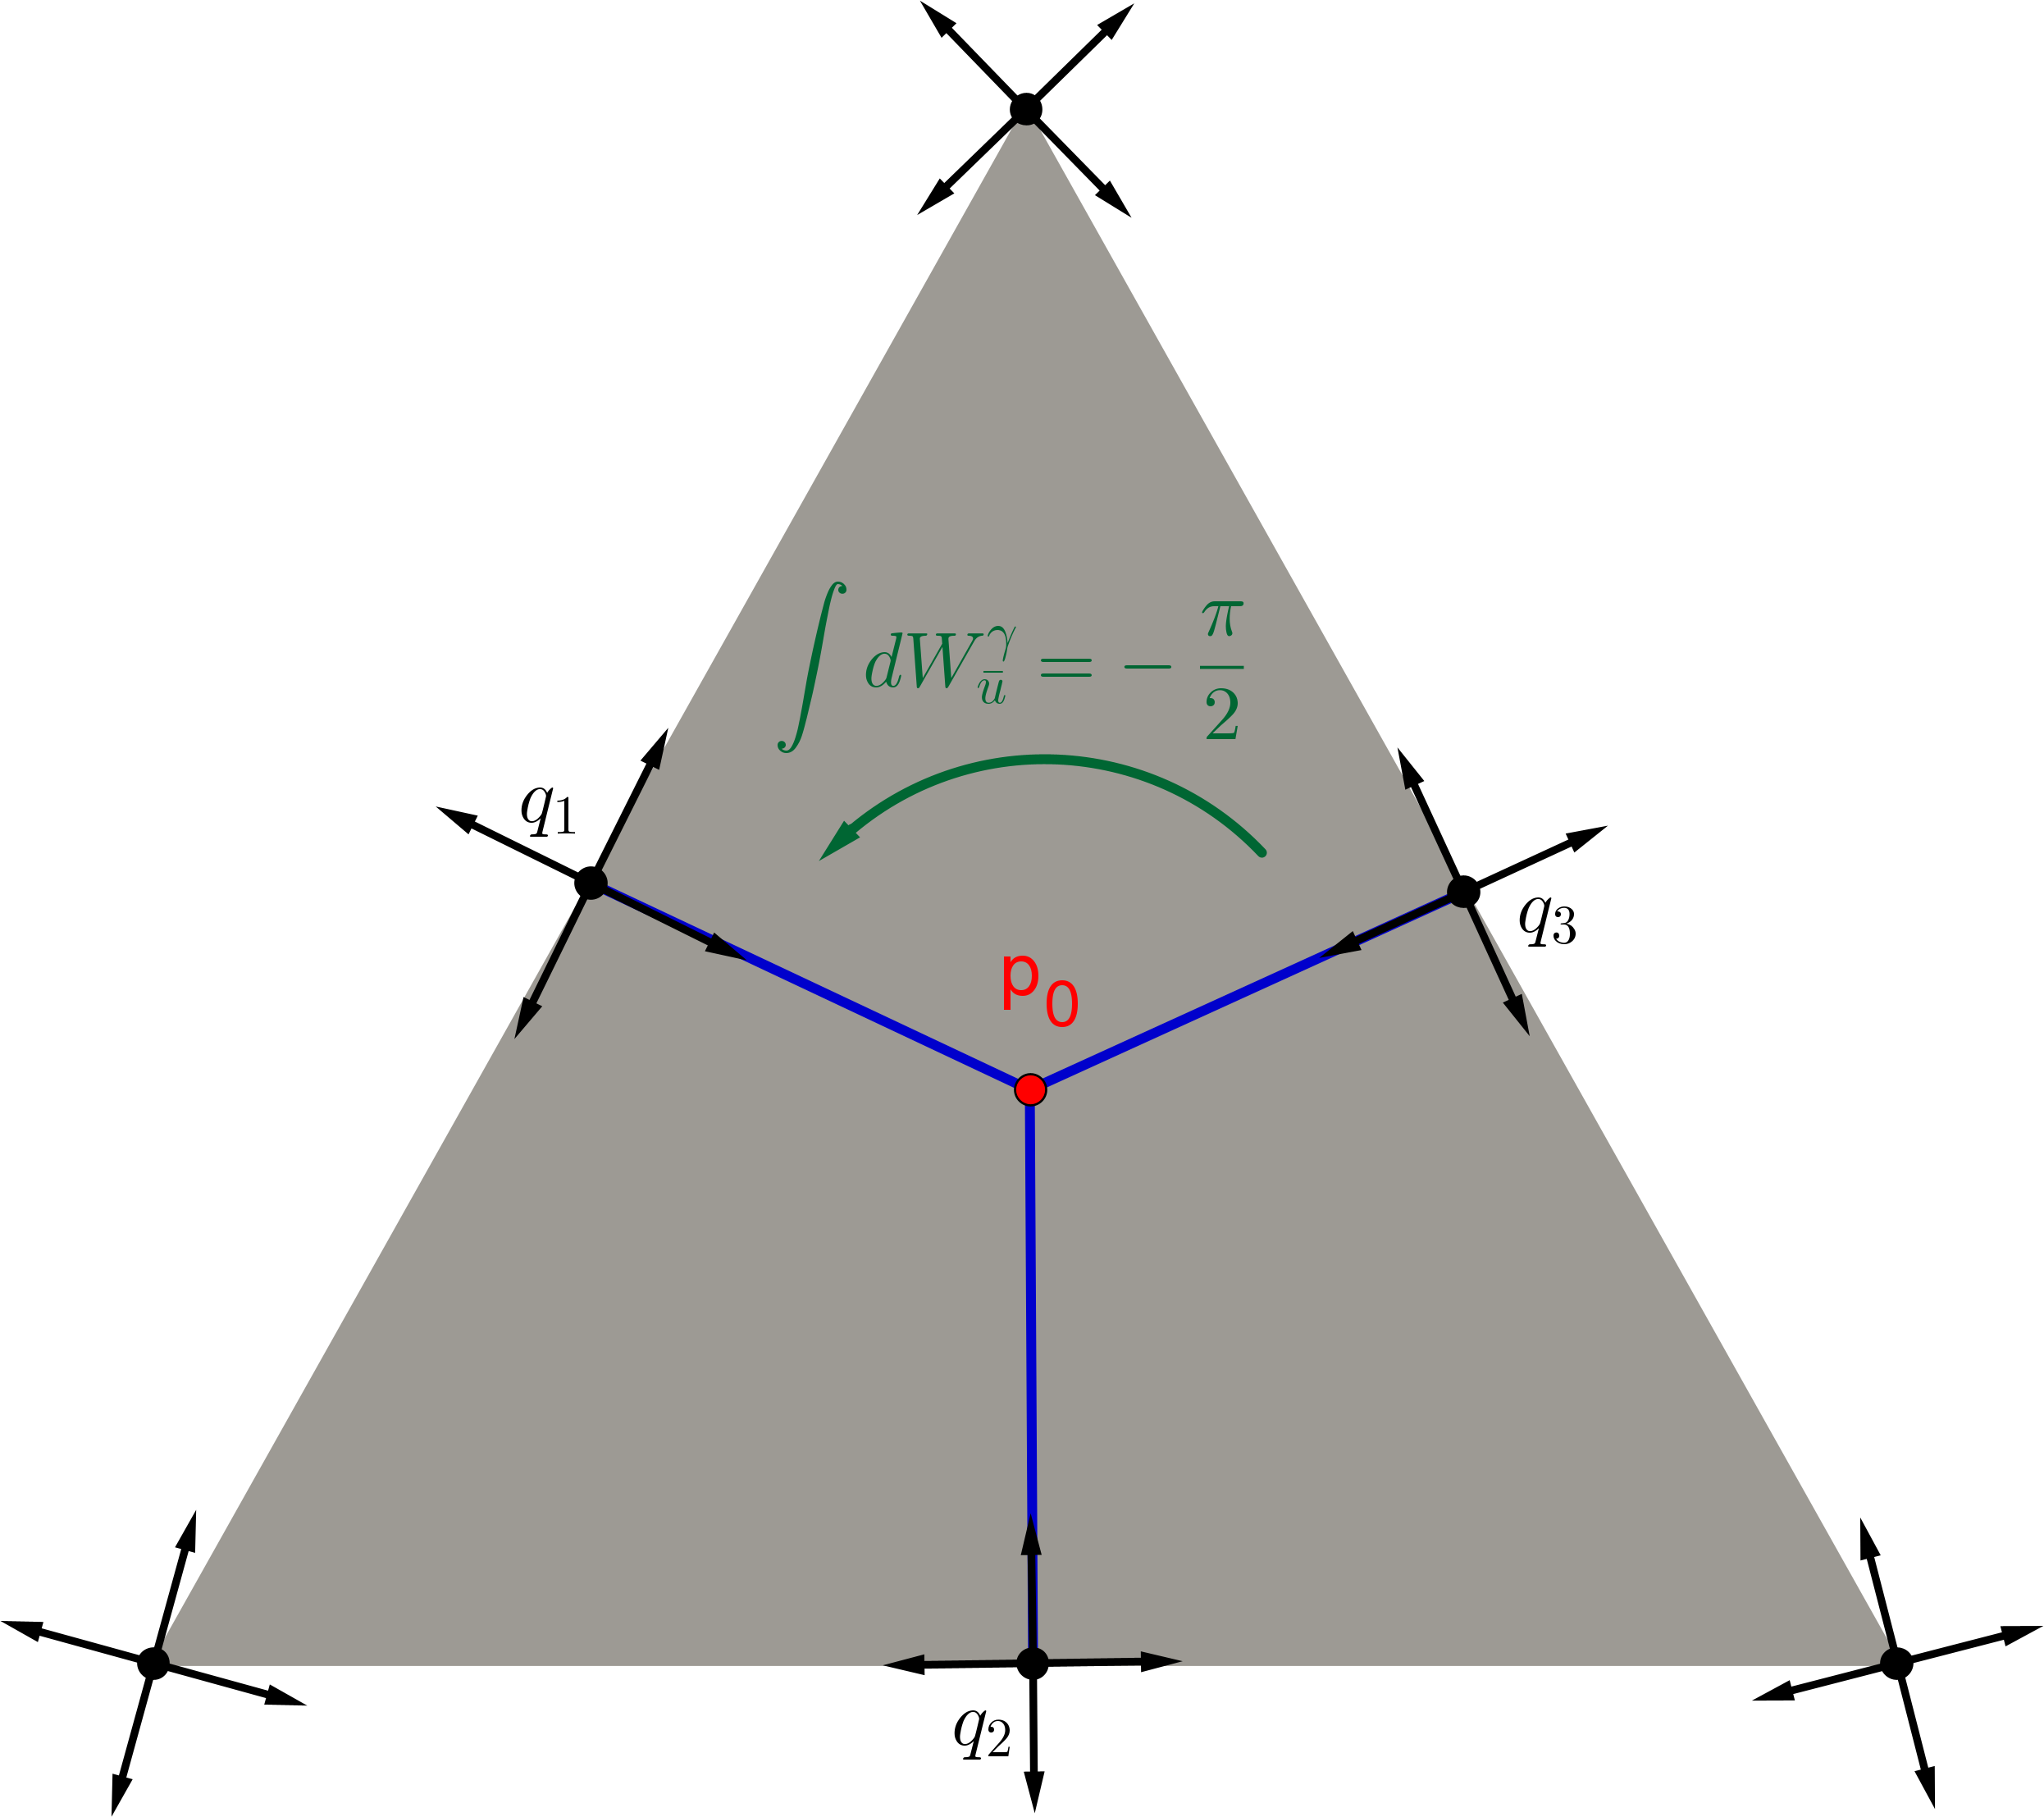
\includegraphics[width=\textwidth]{images/triangle separatrices 3.png}
         \caption{$y=x$}
         \label{fig:y equals x}
     \end{subfigure}
     \hfill
     \begin{subfigure}[b]{0.49\textwidth}
         \centering
         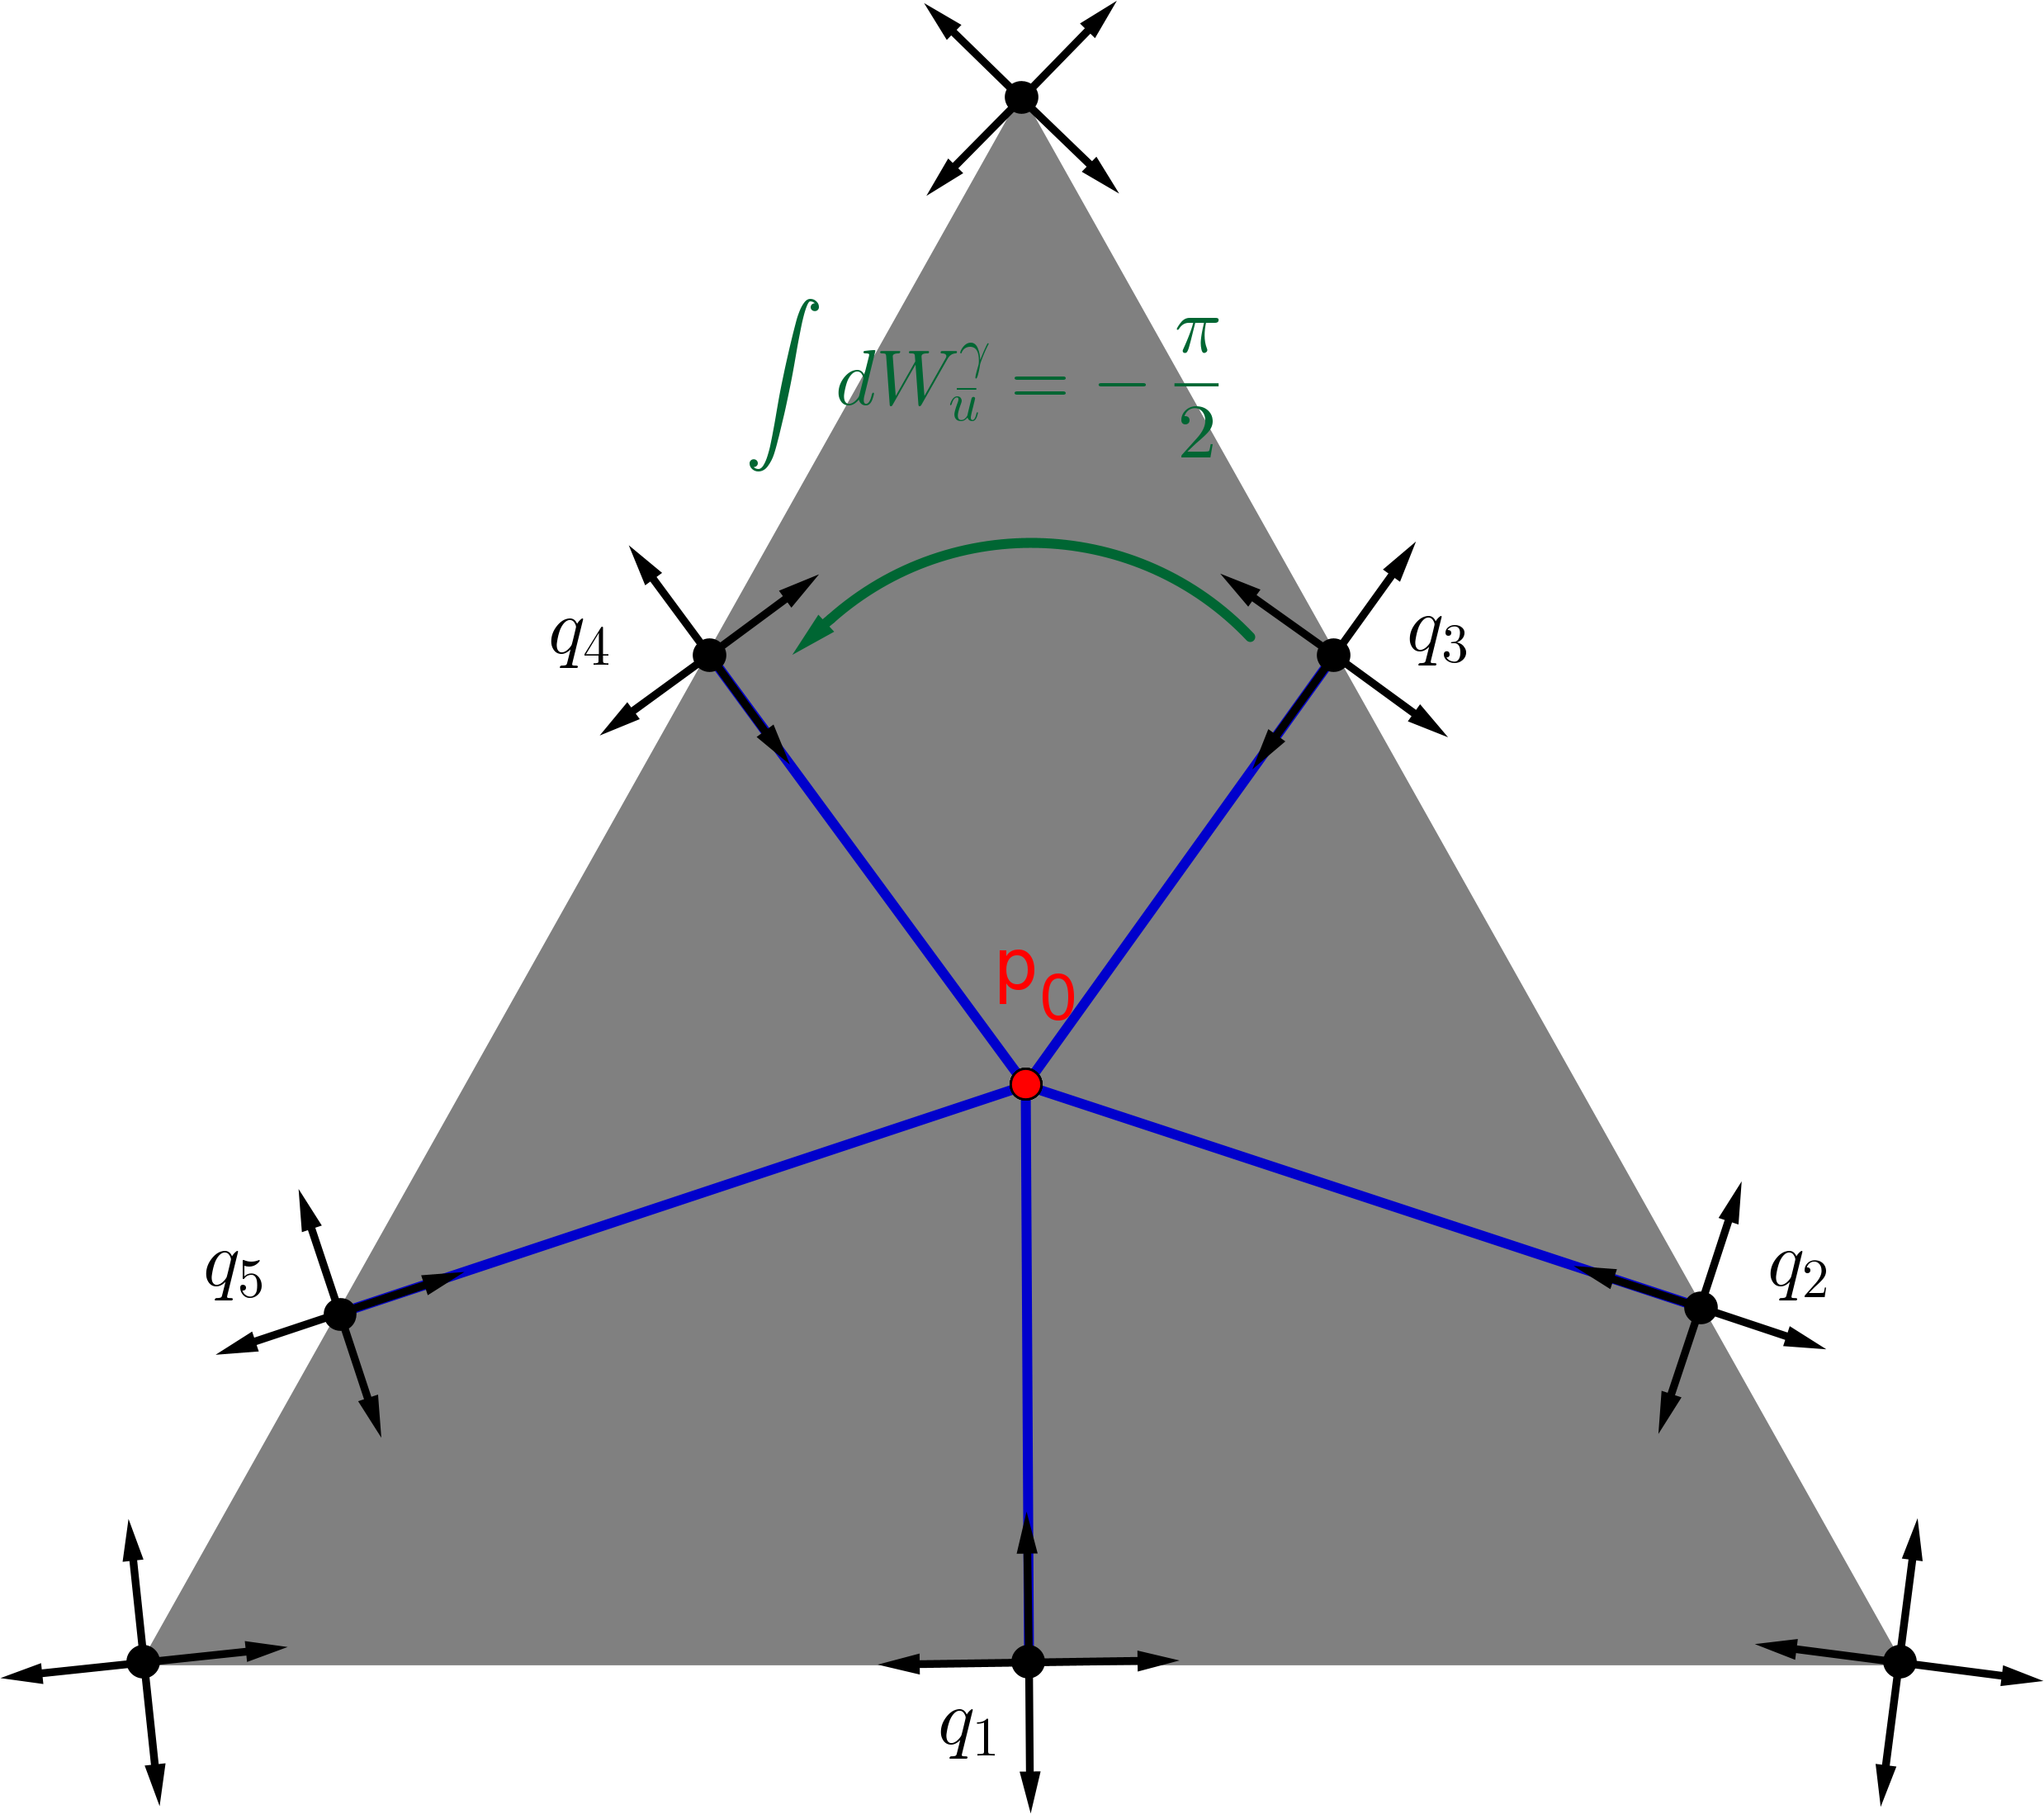
\includegraphics[width=\textwidth]{images/triangle separatrices 5.png}
         \caption{$y=3\sin x$}
         \label{fig:three sin x}
     \end{subfigure}
        \caption{Three simple graphs}
        \label{fig:three graphs}
\end{figure}
On veut etre mesh tri aussi grossier quer possible donc mailler le vrai domaine et non le mesh tri
\paragraph{Intégration des séparatrices:} Considérons $SL_{\bar{u}_h}(p_0,\overrightarrow{p_0p_1})$ la séparatrice émanant de $p_0$ dans la direction du vecteur $\overrightarrow{p_0p_1}$, où $p_1\in\partial F{p_0}$. Nous procédons à la construction d'une approximation $SL^h_{\bar{u}_h}(p_0, \overrightarrow{p_0p_1})$ de $SL_{\bar{u}_h}(p_0, \overrightarrow{p_0p_1})$ sur $\Omega_h$ sous la forme d'une succession de segments. Le premier segment est représenté par $[p_0p_1]$. Ensuite, pour tout $i\geq 1$, on construit le segment  $[p_ip_{i+1}]$ en cherchant le point $p_{i+1}$ comme le point d'intersection entre $\partial F_{p_i}$ et la demi-droite d'origine $p_i$ et dirigée par le vecteur $P(\bar{u}_h(p_i), \overrightarrow{p_{i-1}p_i})+P(\bar{u}_h(p'_{i+1}), \overrightarrow{p_{i-1}p_i})$. Dans cette formule, $p'_{i+1}$ est le point d'intersection entre $\partial F_{p_i}$ et la demi-droite d'origine $p_i$ et dirigé par le vecteur $P(\bar{u}_h(p_i), d_i)$ et pour tout $(\mathbf{c},d)\in\mathbf{C}\backslash\{0\}\times\mathbb{R}^2$, $P(\mathbf{c}, d)$ désigne le vecteur $\mathbf{c}$ qui s'aligne le mieux avec la direction $d$. Autrement dit, il s'agit de l'unique élément de l'ensemble
$$
\left\{c_k~ |~ c_k = \displaystyle\min_{k\in\llbracket 0, 3\rrbracket}|c_k.d-1|\right\}=\underset{c_k\in\mathbf{c},k\in\llbracket1, 4\rrbracket}{\mathrm{argmin}}|c_k.d-1|.
$$
La figure \ref{fig:draw_stream} illustre la construction du segment $[p_ip_{i+1}]$.

\begin{figure}
     \centering
     \begin{subfigure}[b]{0.49\textwidth}
         \centering
         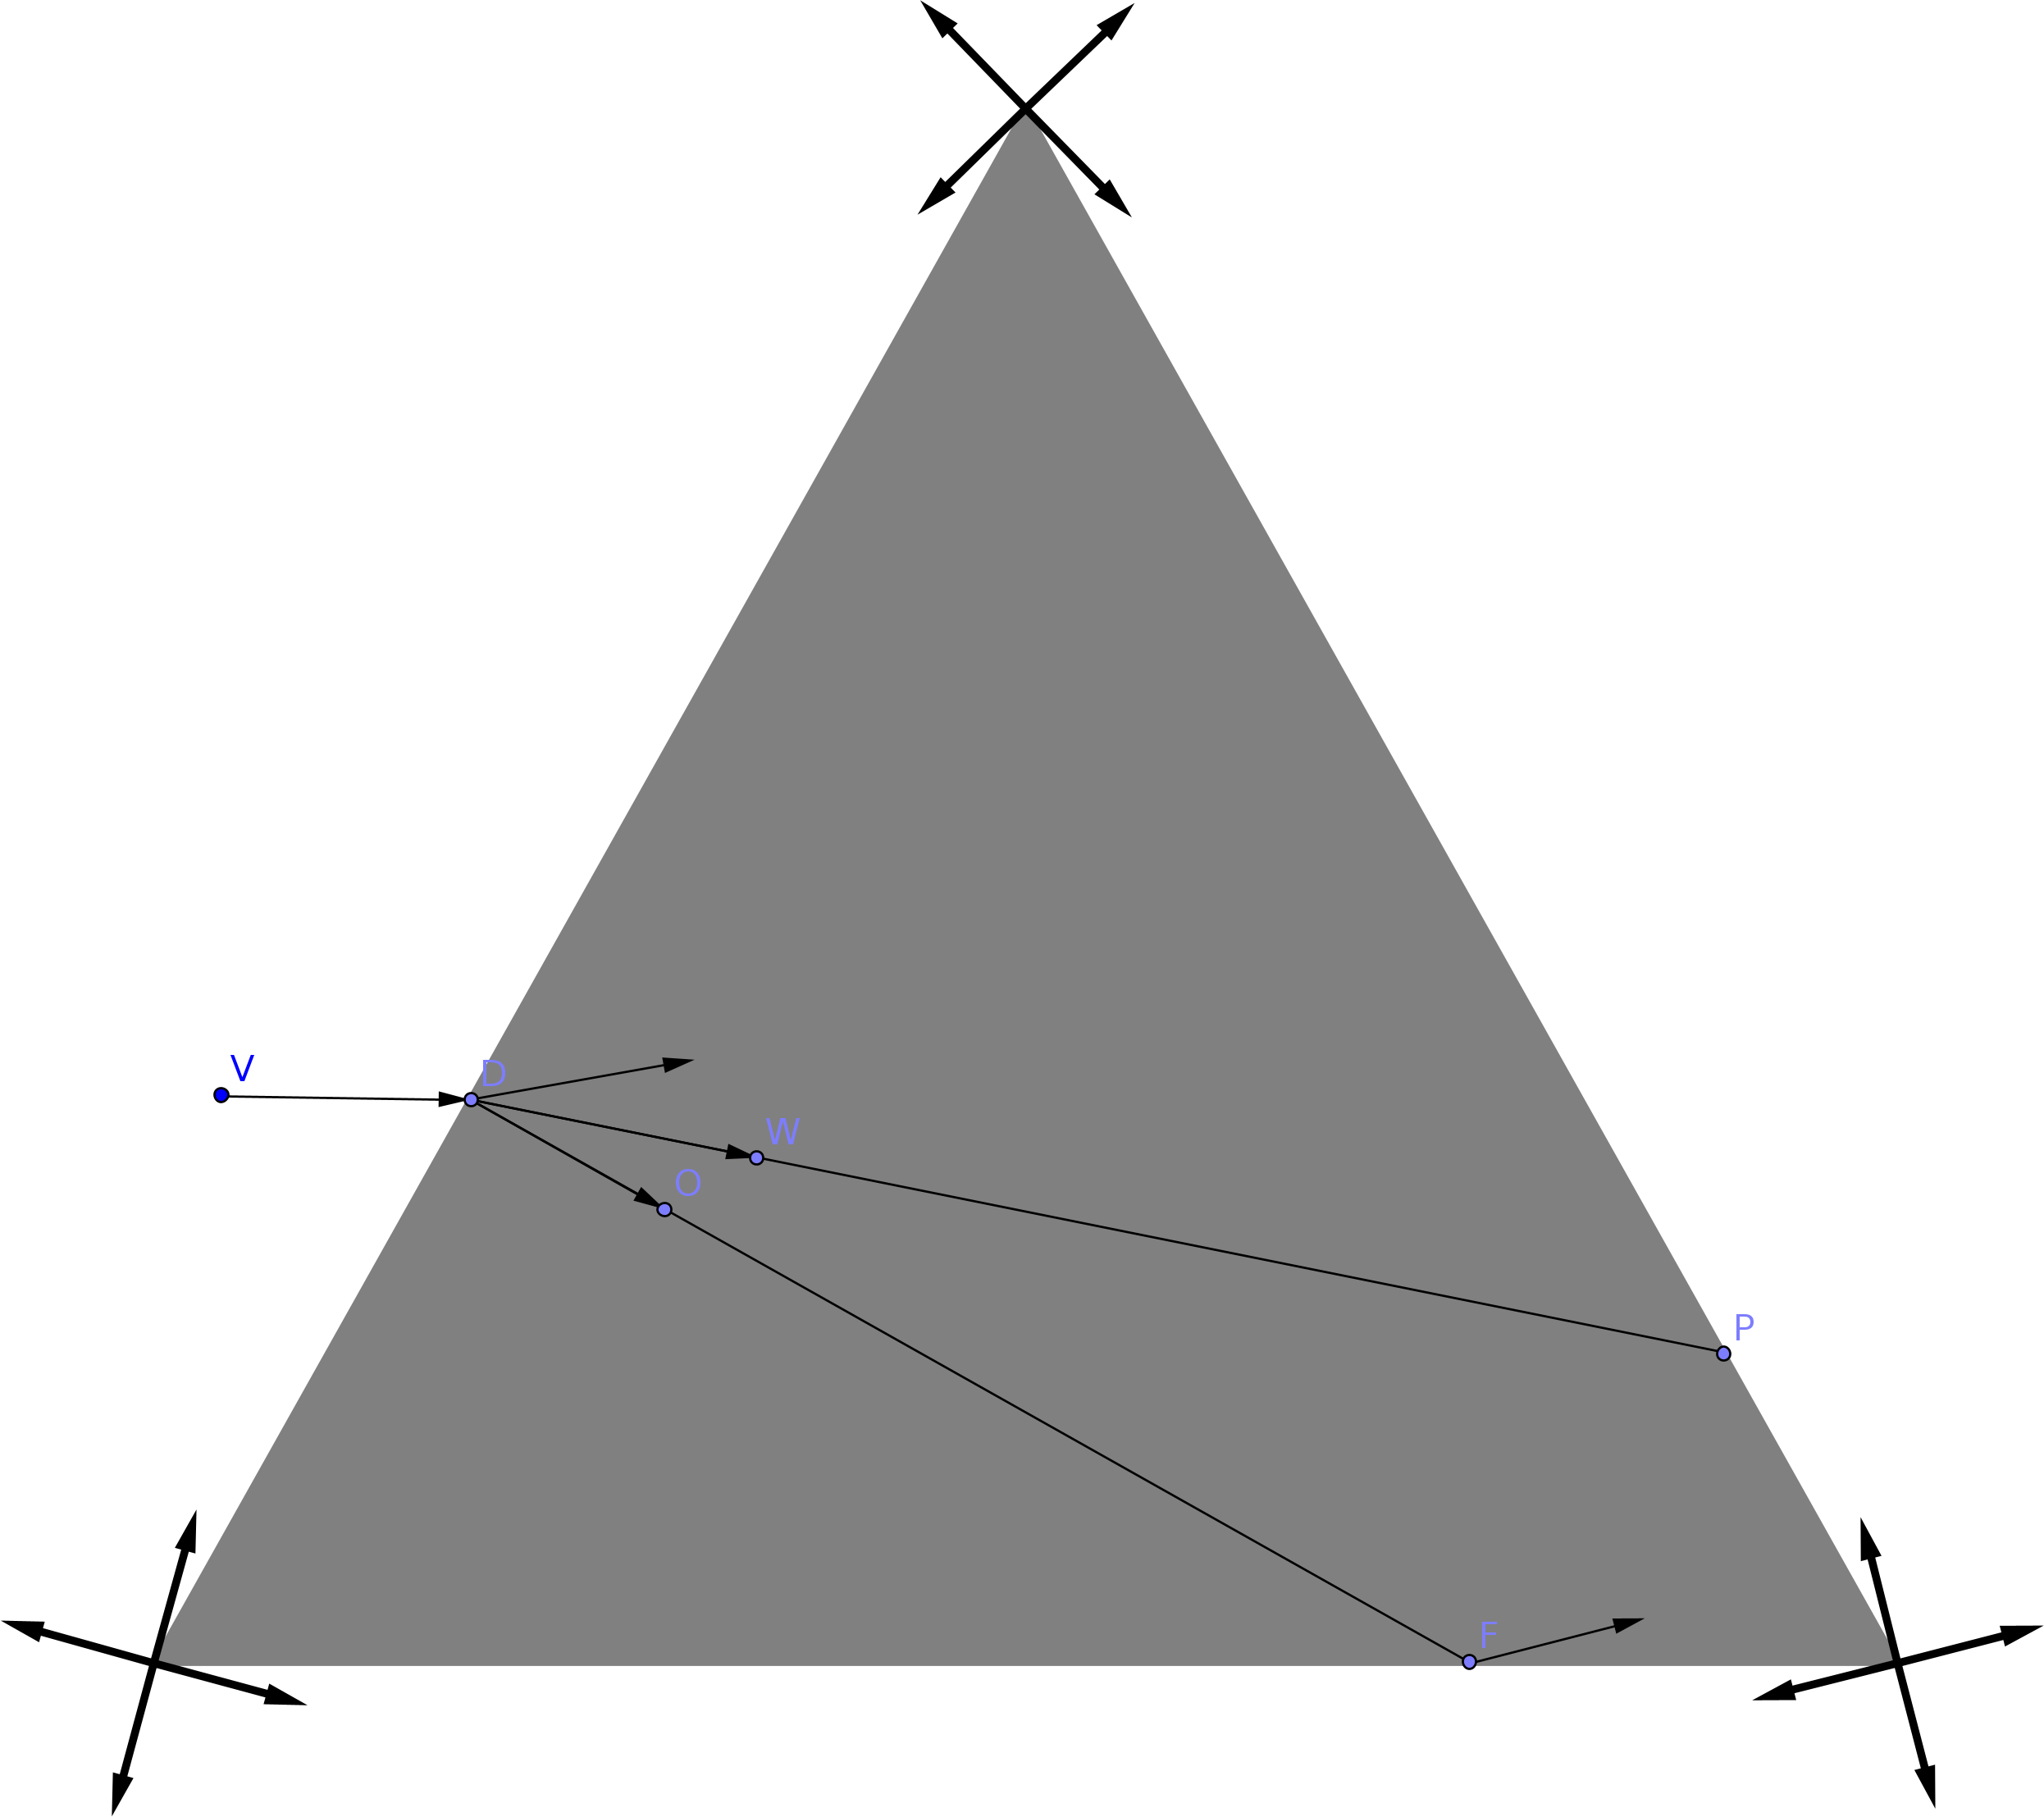
\includegraphics[width=\textwidth]{images/stream_1.png}
         \caption{$y=x$}
         \label{fig:y equals x}
     \end{subfigure}
     \hfill
     \begin{subfigure}[b]{0.49\textwidth}
         \centering
         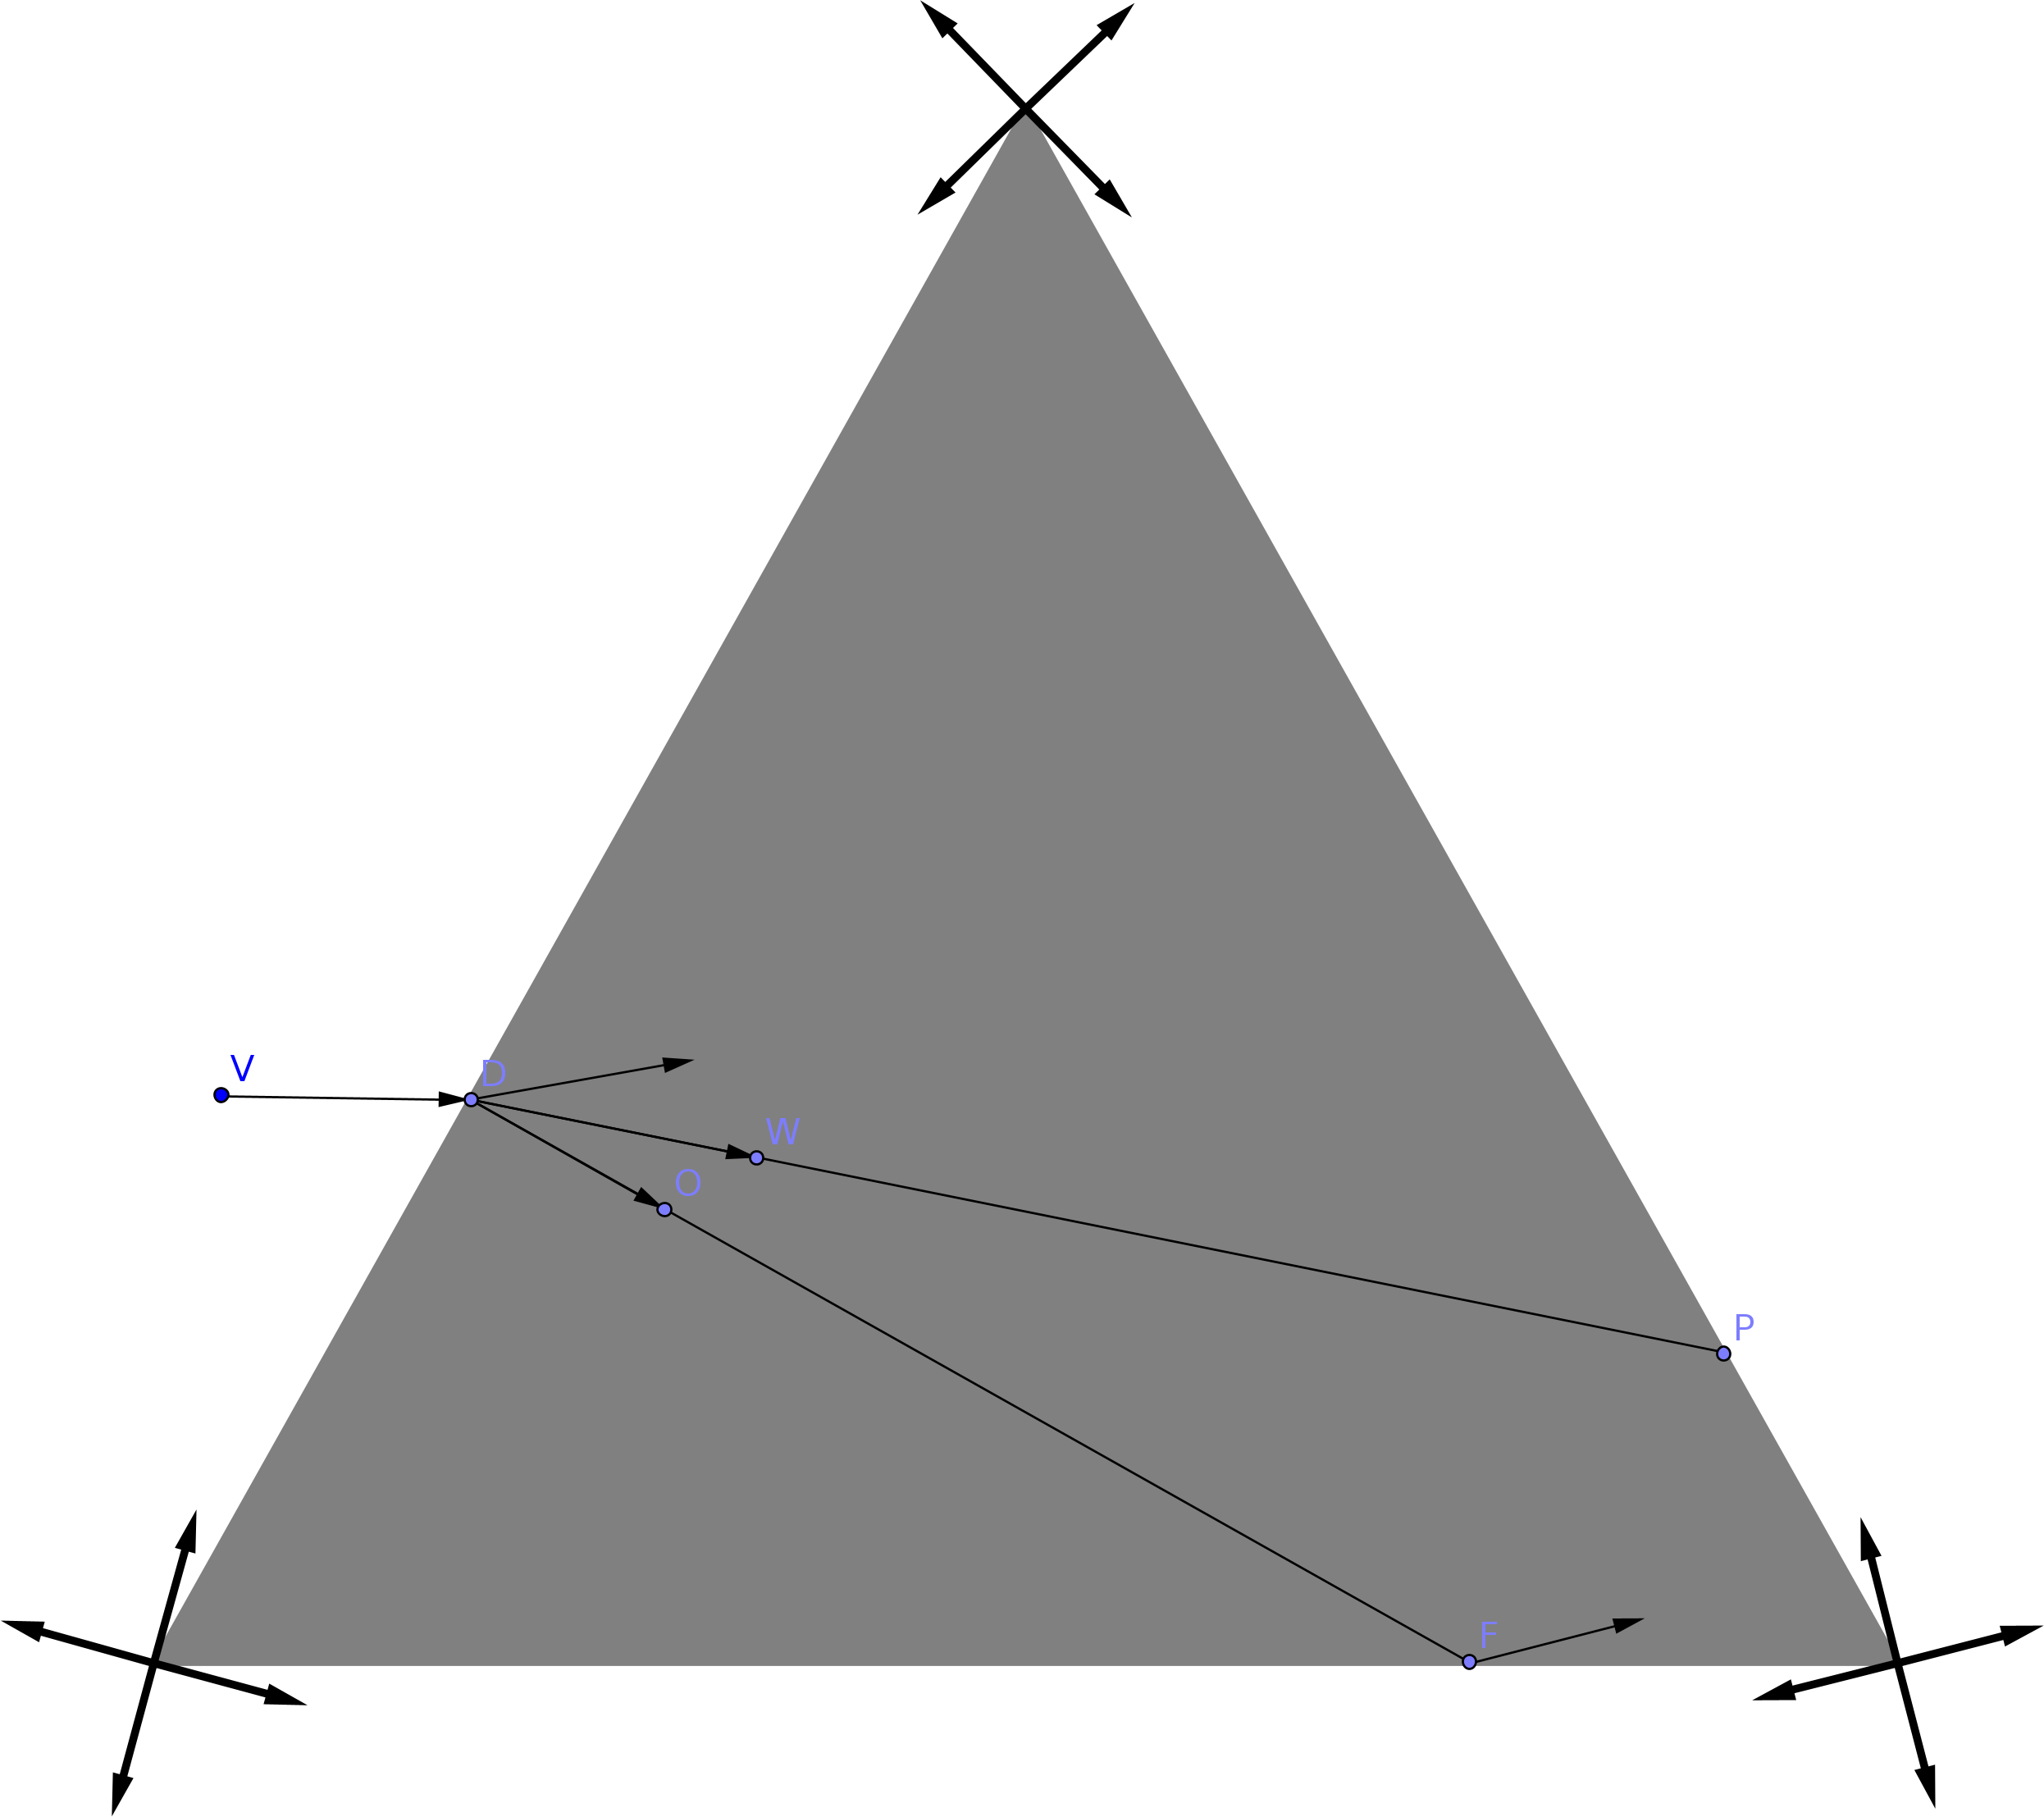
\includegraphics[width=\textwidth]{images/stream_1.png}
         \caption{$y=3\sin x$}
         \label{fig:three sin x}
     \end{subfigure}
        \caption{Three simple graphs}
        \label{fig:draw_stream}
\end{figure}


direction de sortie mieux chez moi que chez les autres

\begin{figure}[!h]
\centering
\begin{subfigure}{0.65\textwidth}
    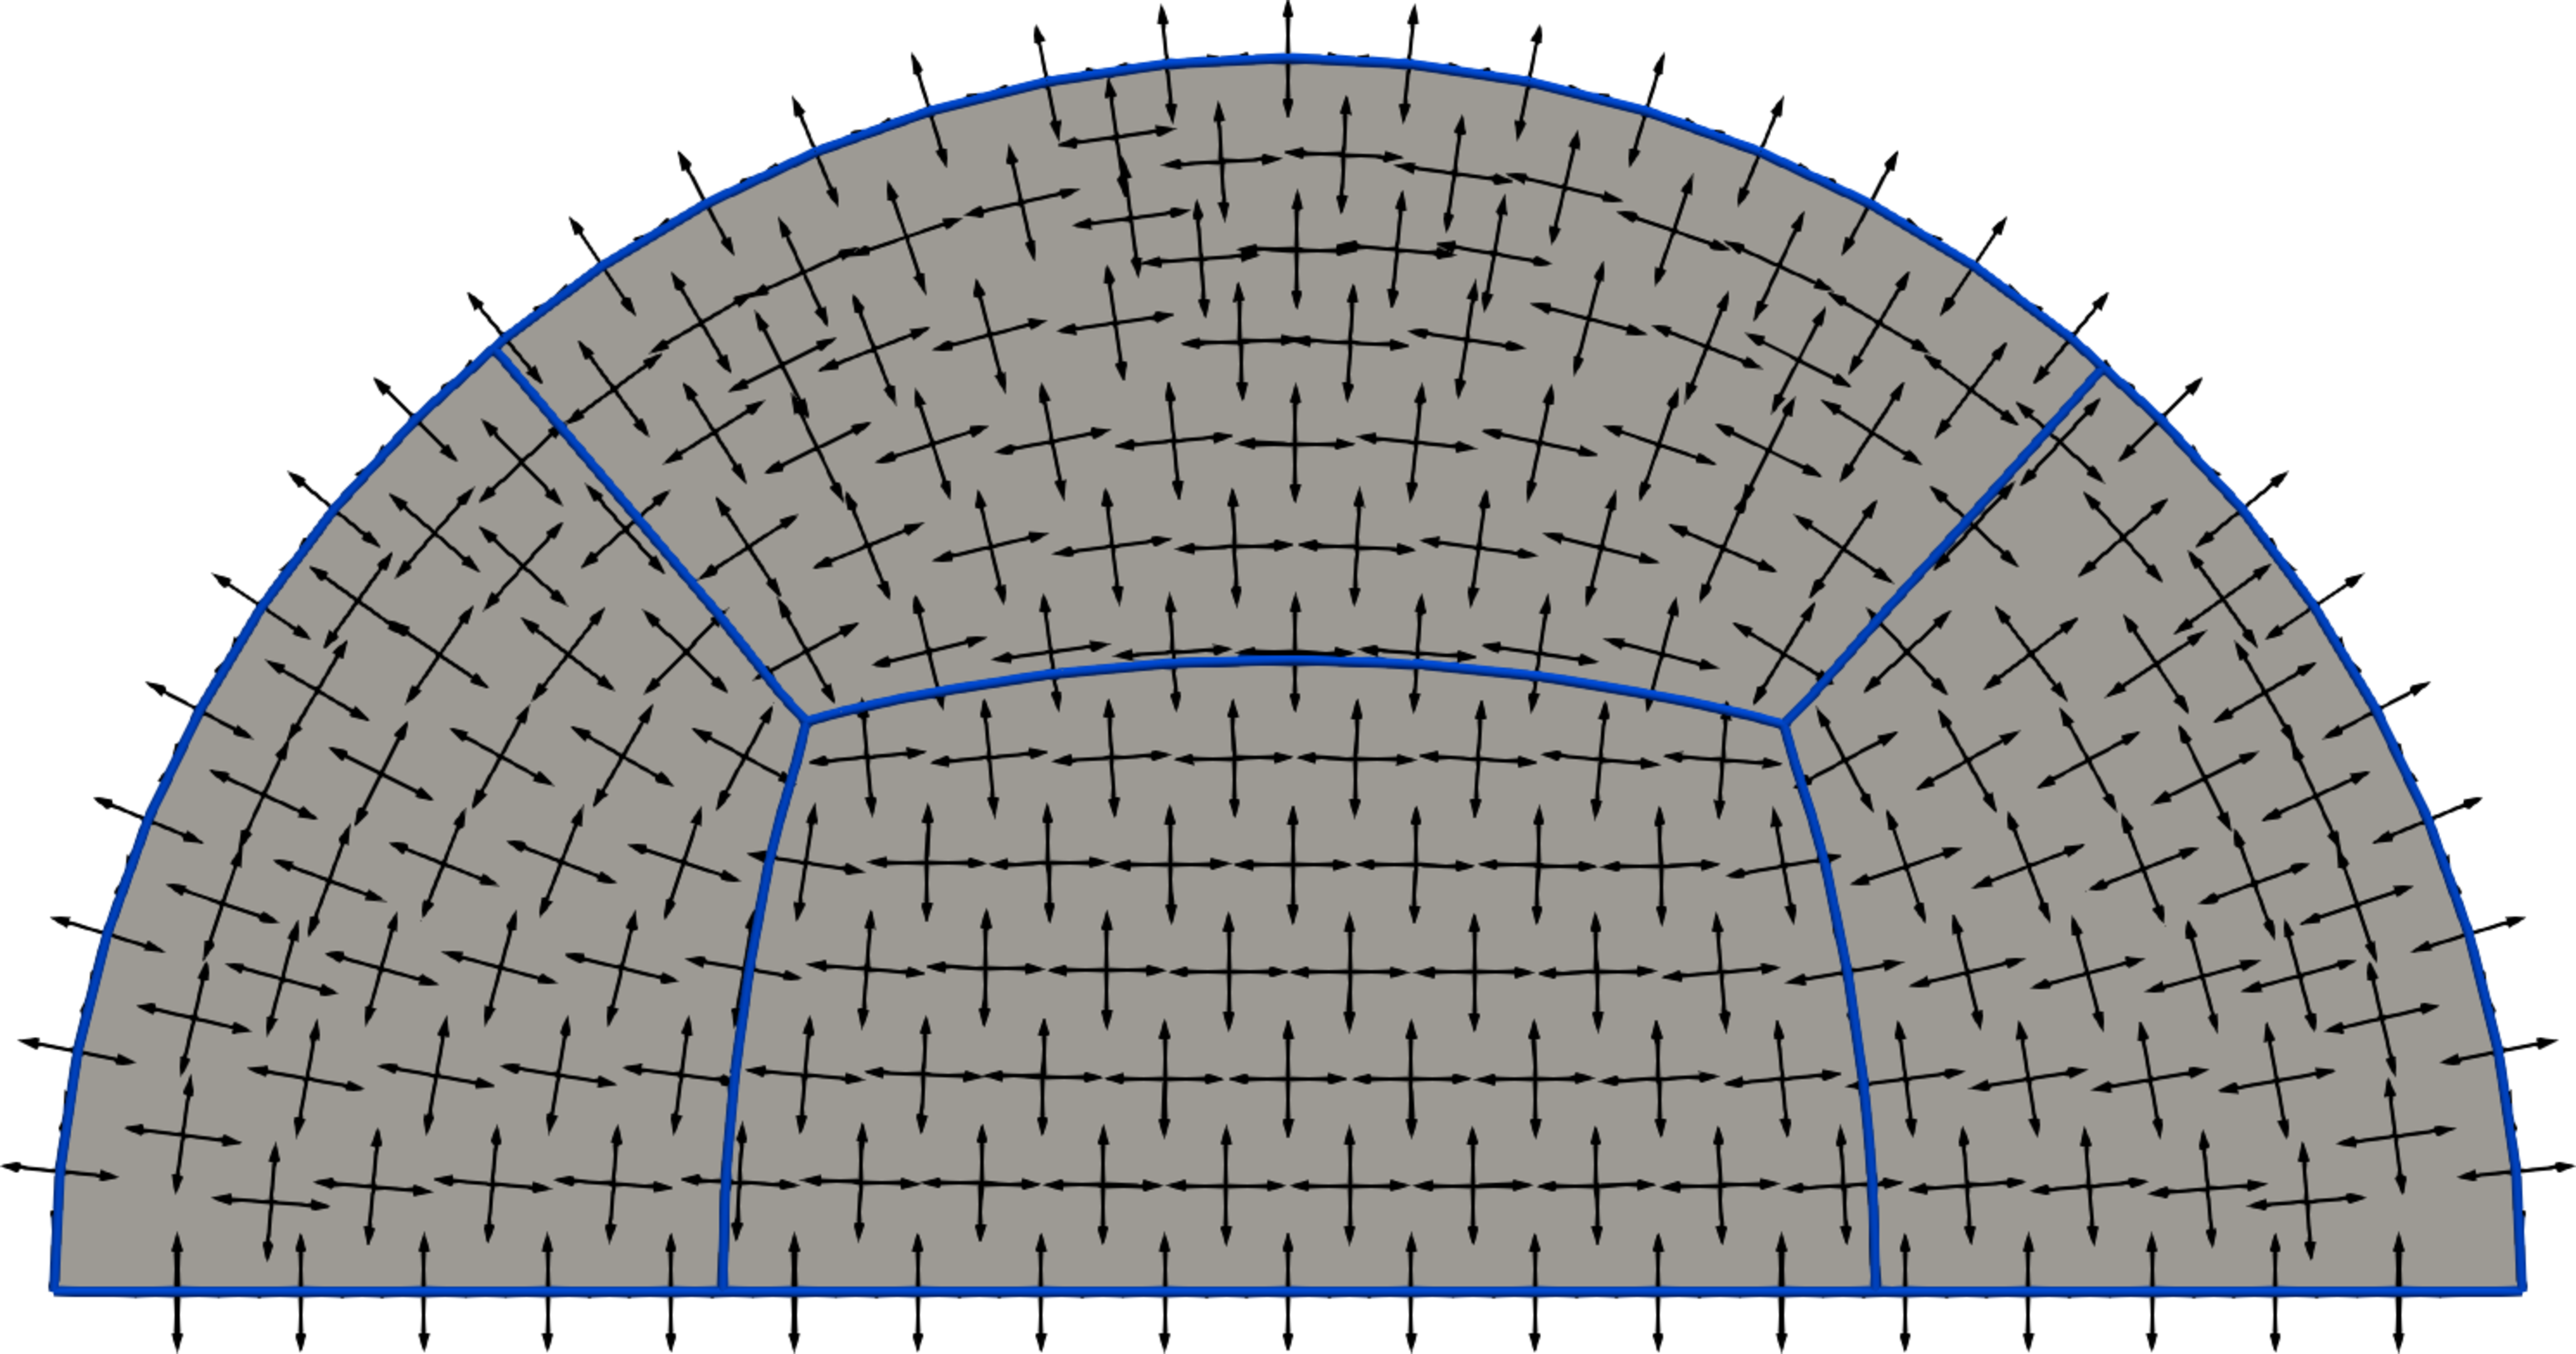
\includegraphics[width=\textwidth]{images/demi_disc_second_phi_first.pdf}
    \caption{Alignement du champ de croix présenté sur la figure \ref{fig:demiDisc_valProp_mauvaix_decoup} sur le bord du domaine et partitionnement du domaine.}
    \label{fig:first_dir_first}
\end{subfigure}
\\[0.5cm]
\begin{subfigure}{0.65\textwidth}
    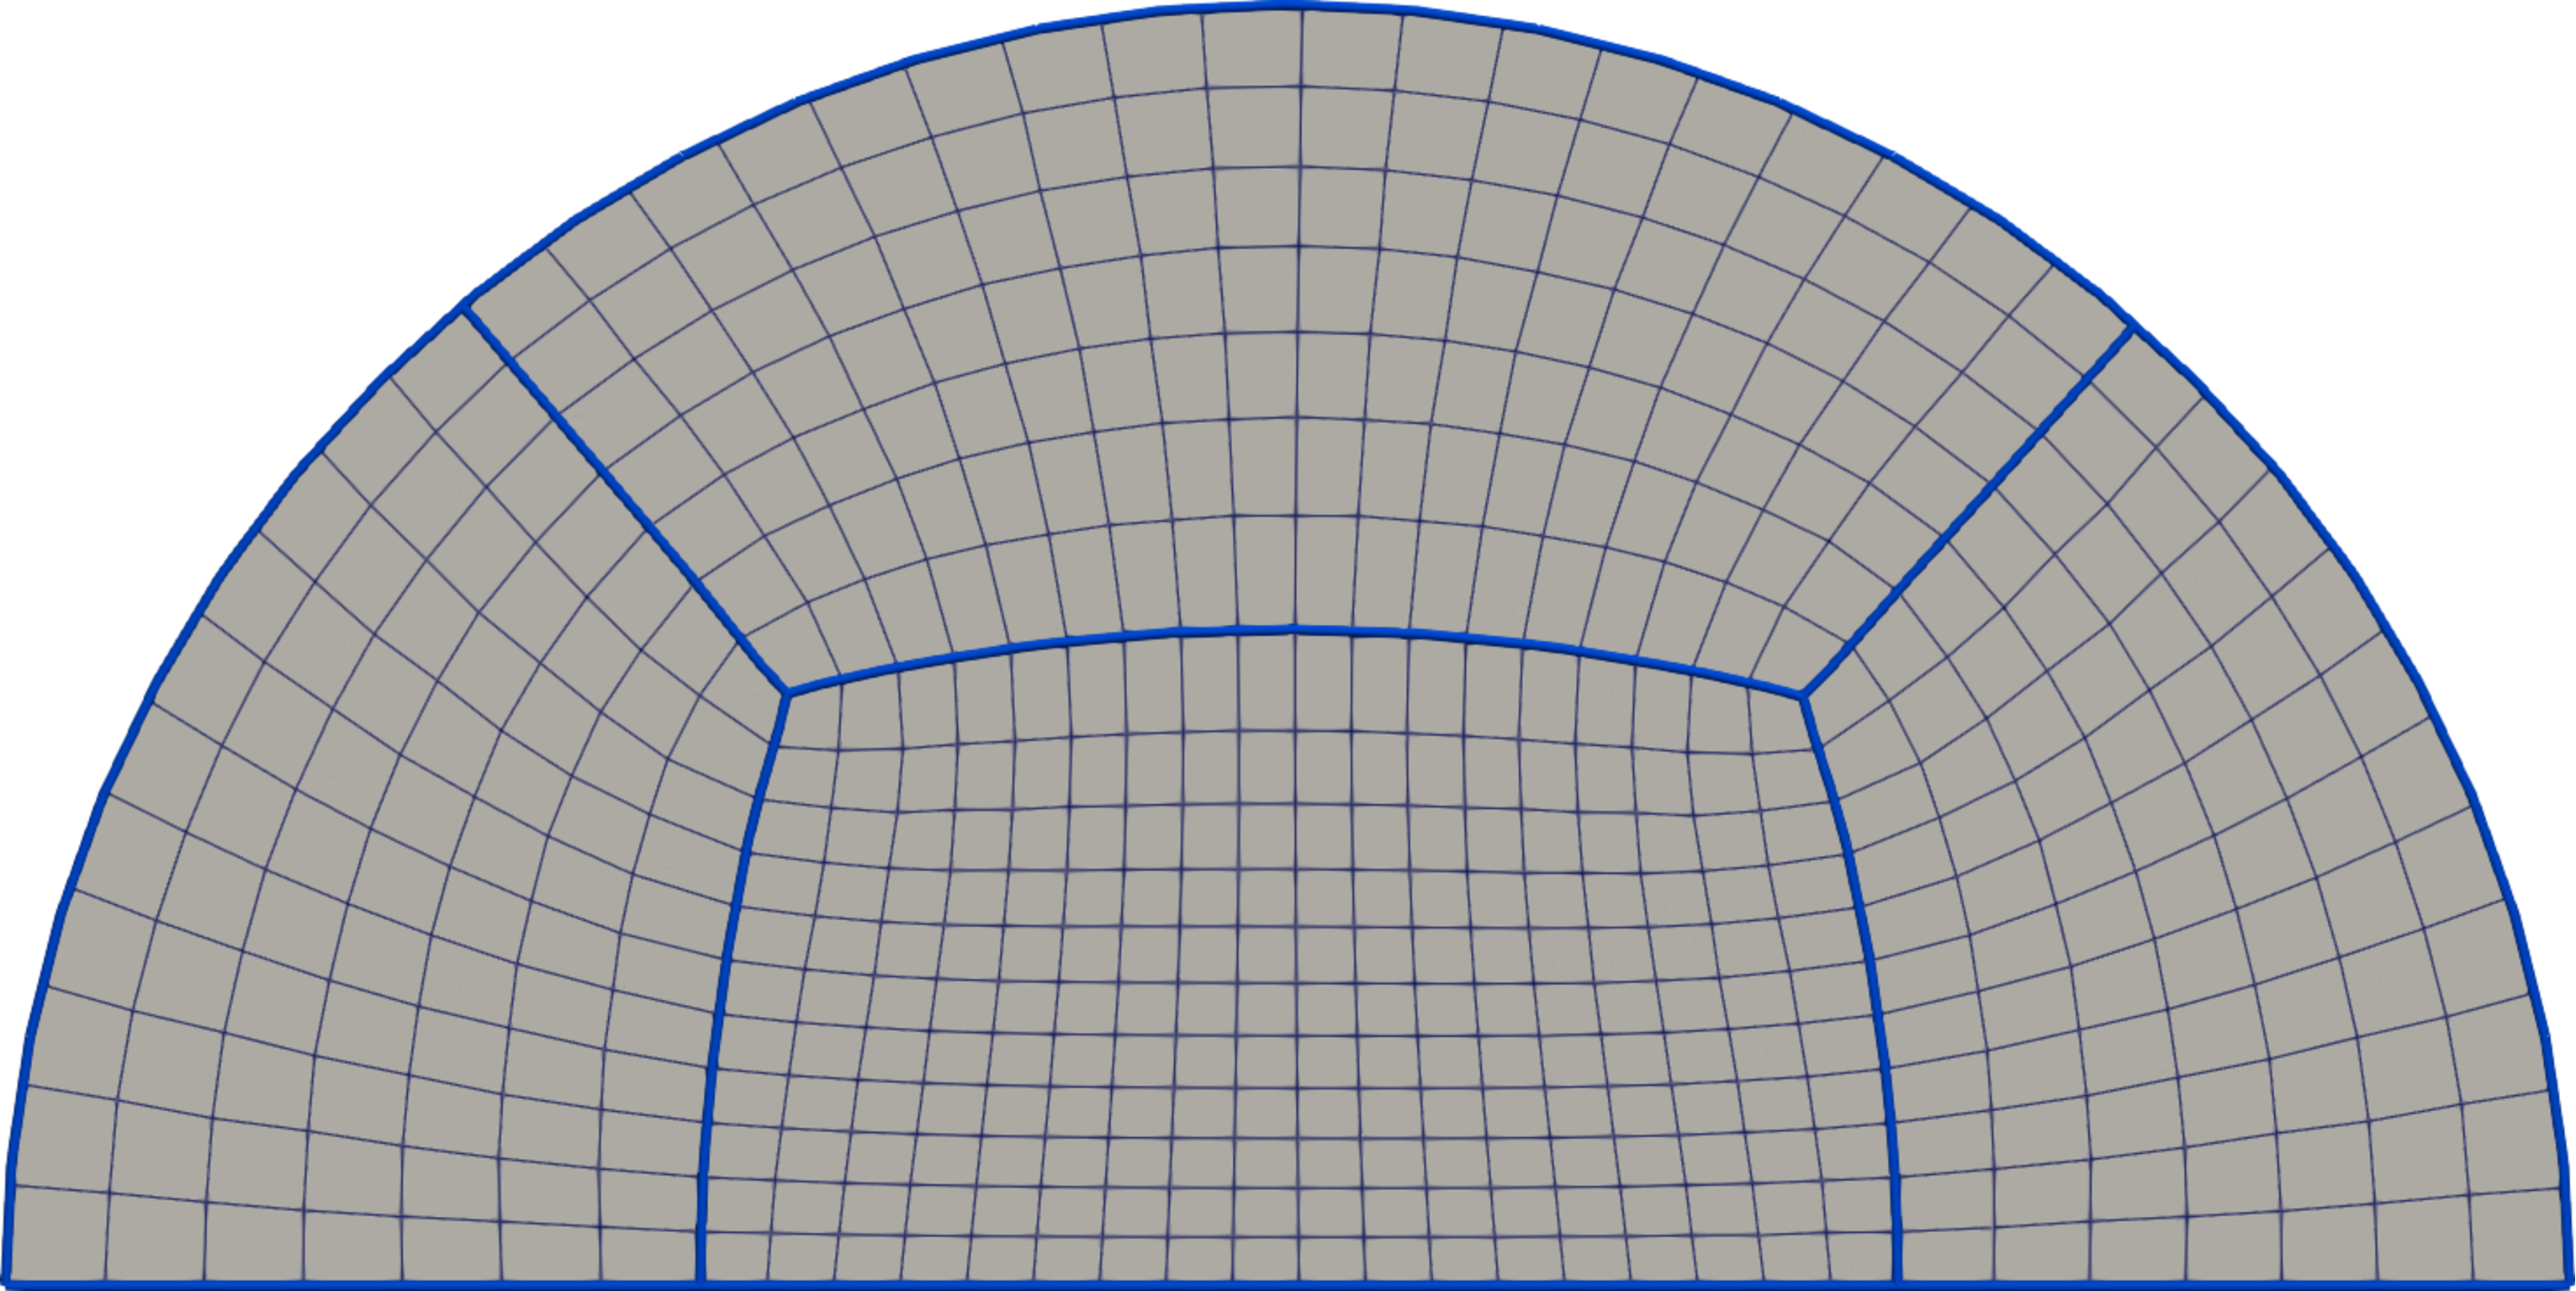
\includegraphics[width=\textwidth]{images/demi_disc_second_phi_second.pdf}
    \caption{Maillage quadrilatéral du domaine.}
    \label{fig:first_dir_second}
\end{subfigure}        
\caption{Direction de sortie différentes.}
\label{fig:first_dir}
\end{figure}


\paragraph{Traversé d'un triangle singulier:} lorsque le segment $[p_ip_{i+1}]$ traverse un triangle singulier, l'angle du champ varie beaucoup. On remplace alors le segment en question par une succecion d'autre segment calculé en raffinant localement le maillage dans le triangle singulier.

\paragraph{Fusion de séparatrices:} 
De manière similaire à ce qui est réalisé dans \cite{marcon2019high}, les séparatrices du champ de croix sont construites simultanément en incrémentant chacune d'elles progressivement, et la rencontre entre deux séparatrices est anticipée en comparant à chaque incrément, d'une part, la distance entre les derniers points calculés et, d'autre part, les directions des derniers segments construits. En d'autres termes, on cherche à déterminer si, à un moment donné, deux séparatrices données avancent dans des directions opposées et si elles sont suffisamment proches l'une de l'autre. On compare ces deux mesures à des seuils prédéfinis, et en fonction du résultat, on décide de fusionner ou non les deux séparatrices.

La fusion se réalise en créant une nouvelle séparatrice par une fusion linéaire des points des deux séparatrices impliquées. Pour se faire, chaque séparatrice est prolongée à travers $\Omega_h$ jusqu'à atteindre la position de départ de l'autre, tout en maintenant le même nombre de points pour chacune des séparatrices. L'intérêt de fusionner les séparatrices réside dans la réduction de leur nombre, ce qui se traduit directement par une diminution du nombre de régions générées lors du découpage du domaine. Nous illustrons la fusion de deux séparatrices sur la figure \ref{fig:merge_sepa}. On observe sur que la non fusion donne plus de region qui sont notemment tres etirer et non homogene par rapport aux autres ce qui induit des mesh quad non homogene.

\begin{figure}[!h]
\centering
\begin{subfigure}{0.65\textwidth}
    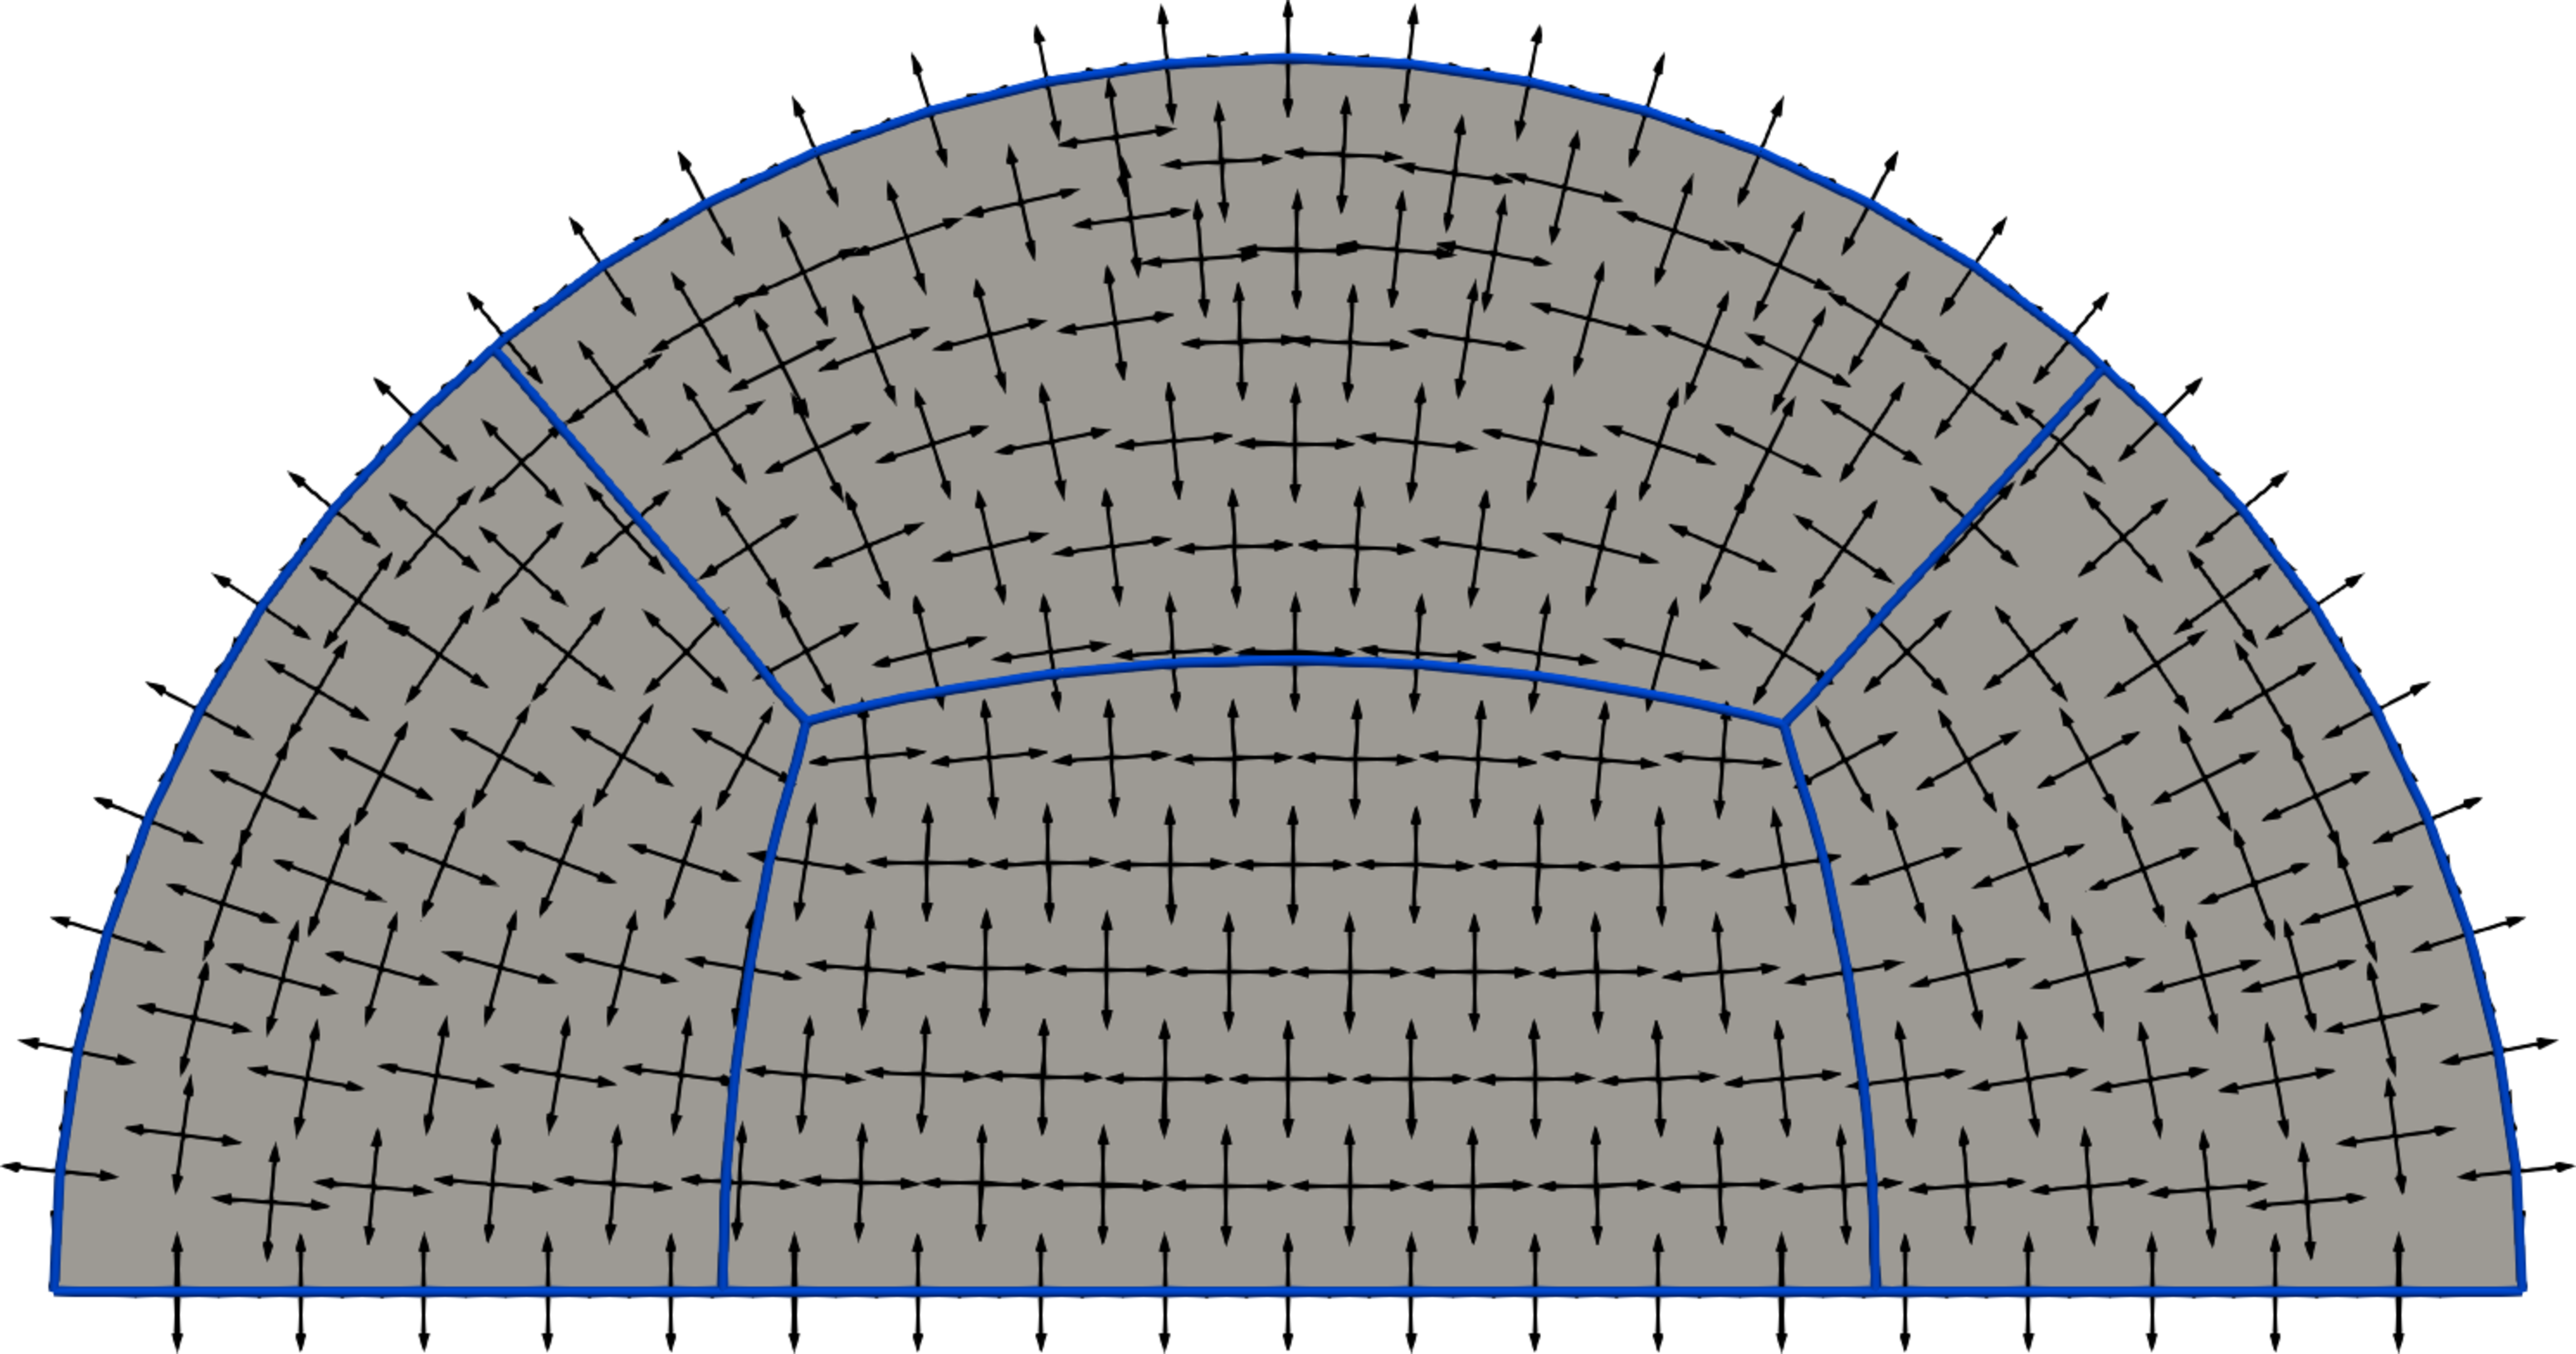
\includegraphics[width=\textwidth]{images/demi_disc_second_phi_first.pdf}
    \caption{Sans fusion}
    \label{fig:merge_sepa_first}
\end{subfigure}
\\[0.5cm]
\begin{subfigure}{0.65\textwidth}
    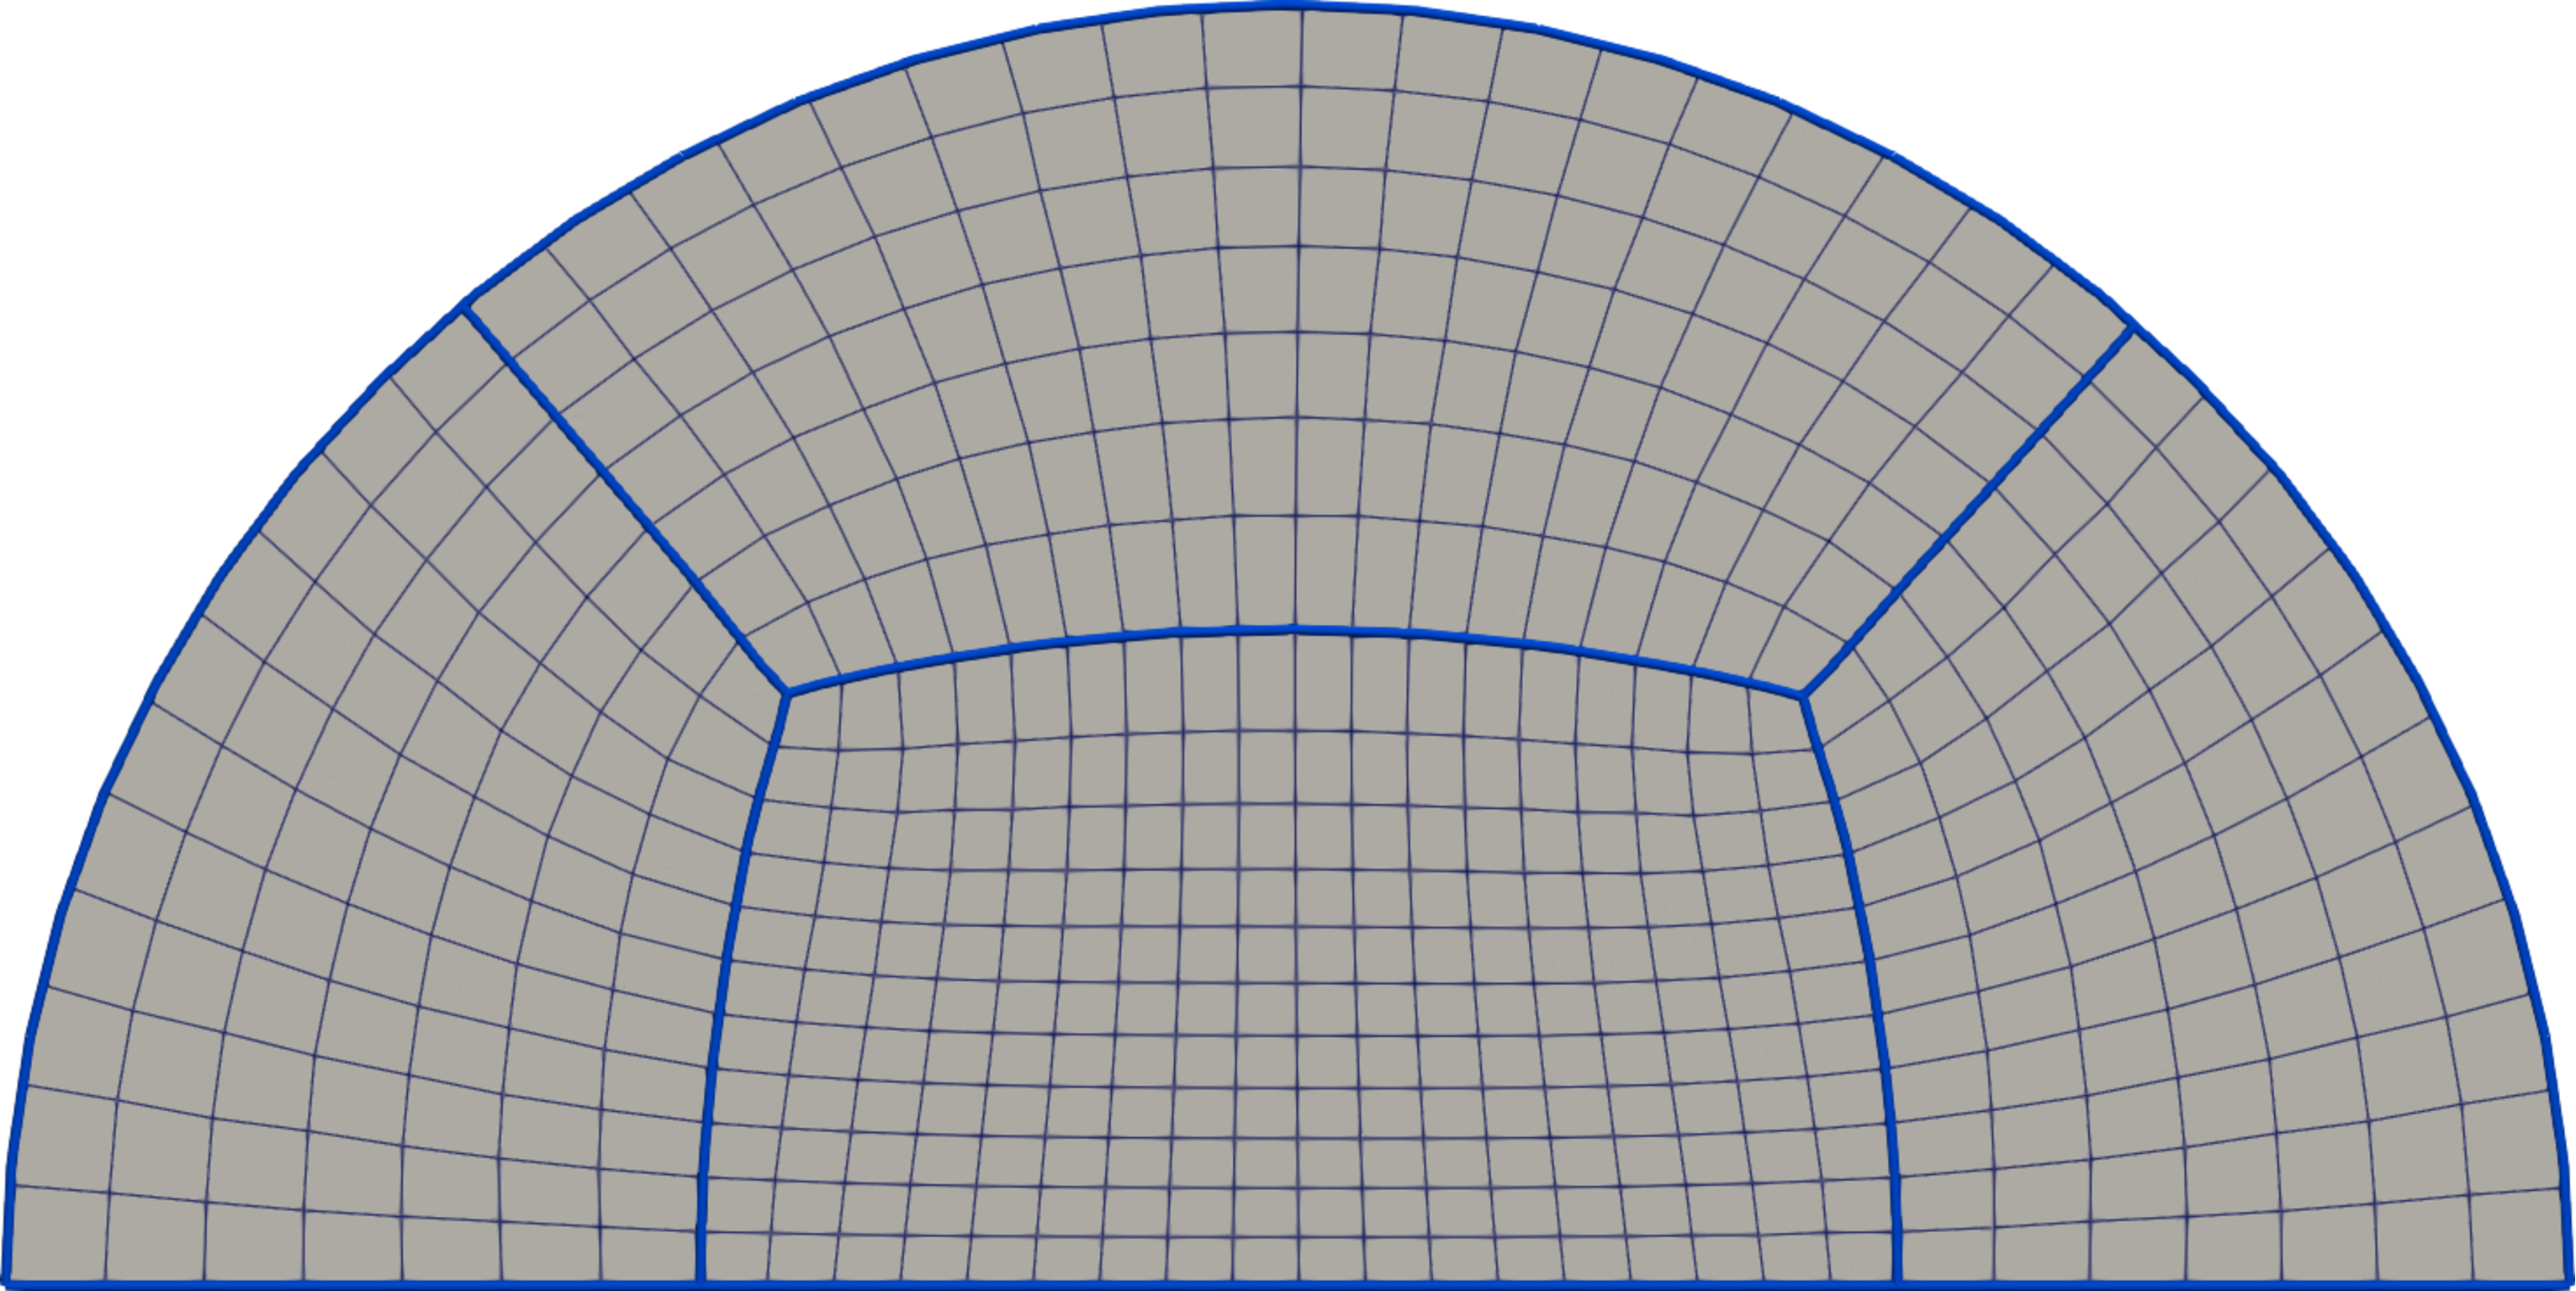
\includegraphics[width=\textwidth]{images/demi_disc_second_phi_second.pdf}
    \caption{detection fusion.}
    \label{fig:merge_sepa_second}
\end{subfigure}        
\\[0.5cm]
\begin{subfigure}{0.65\textwidth}
    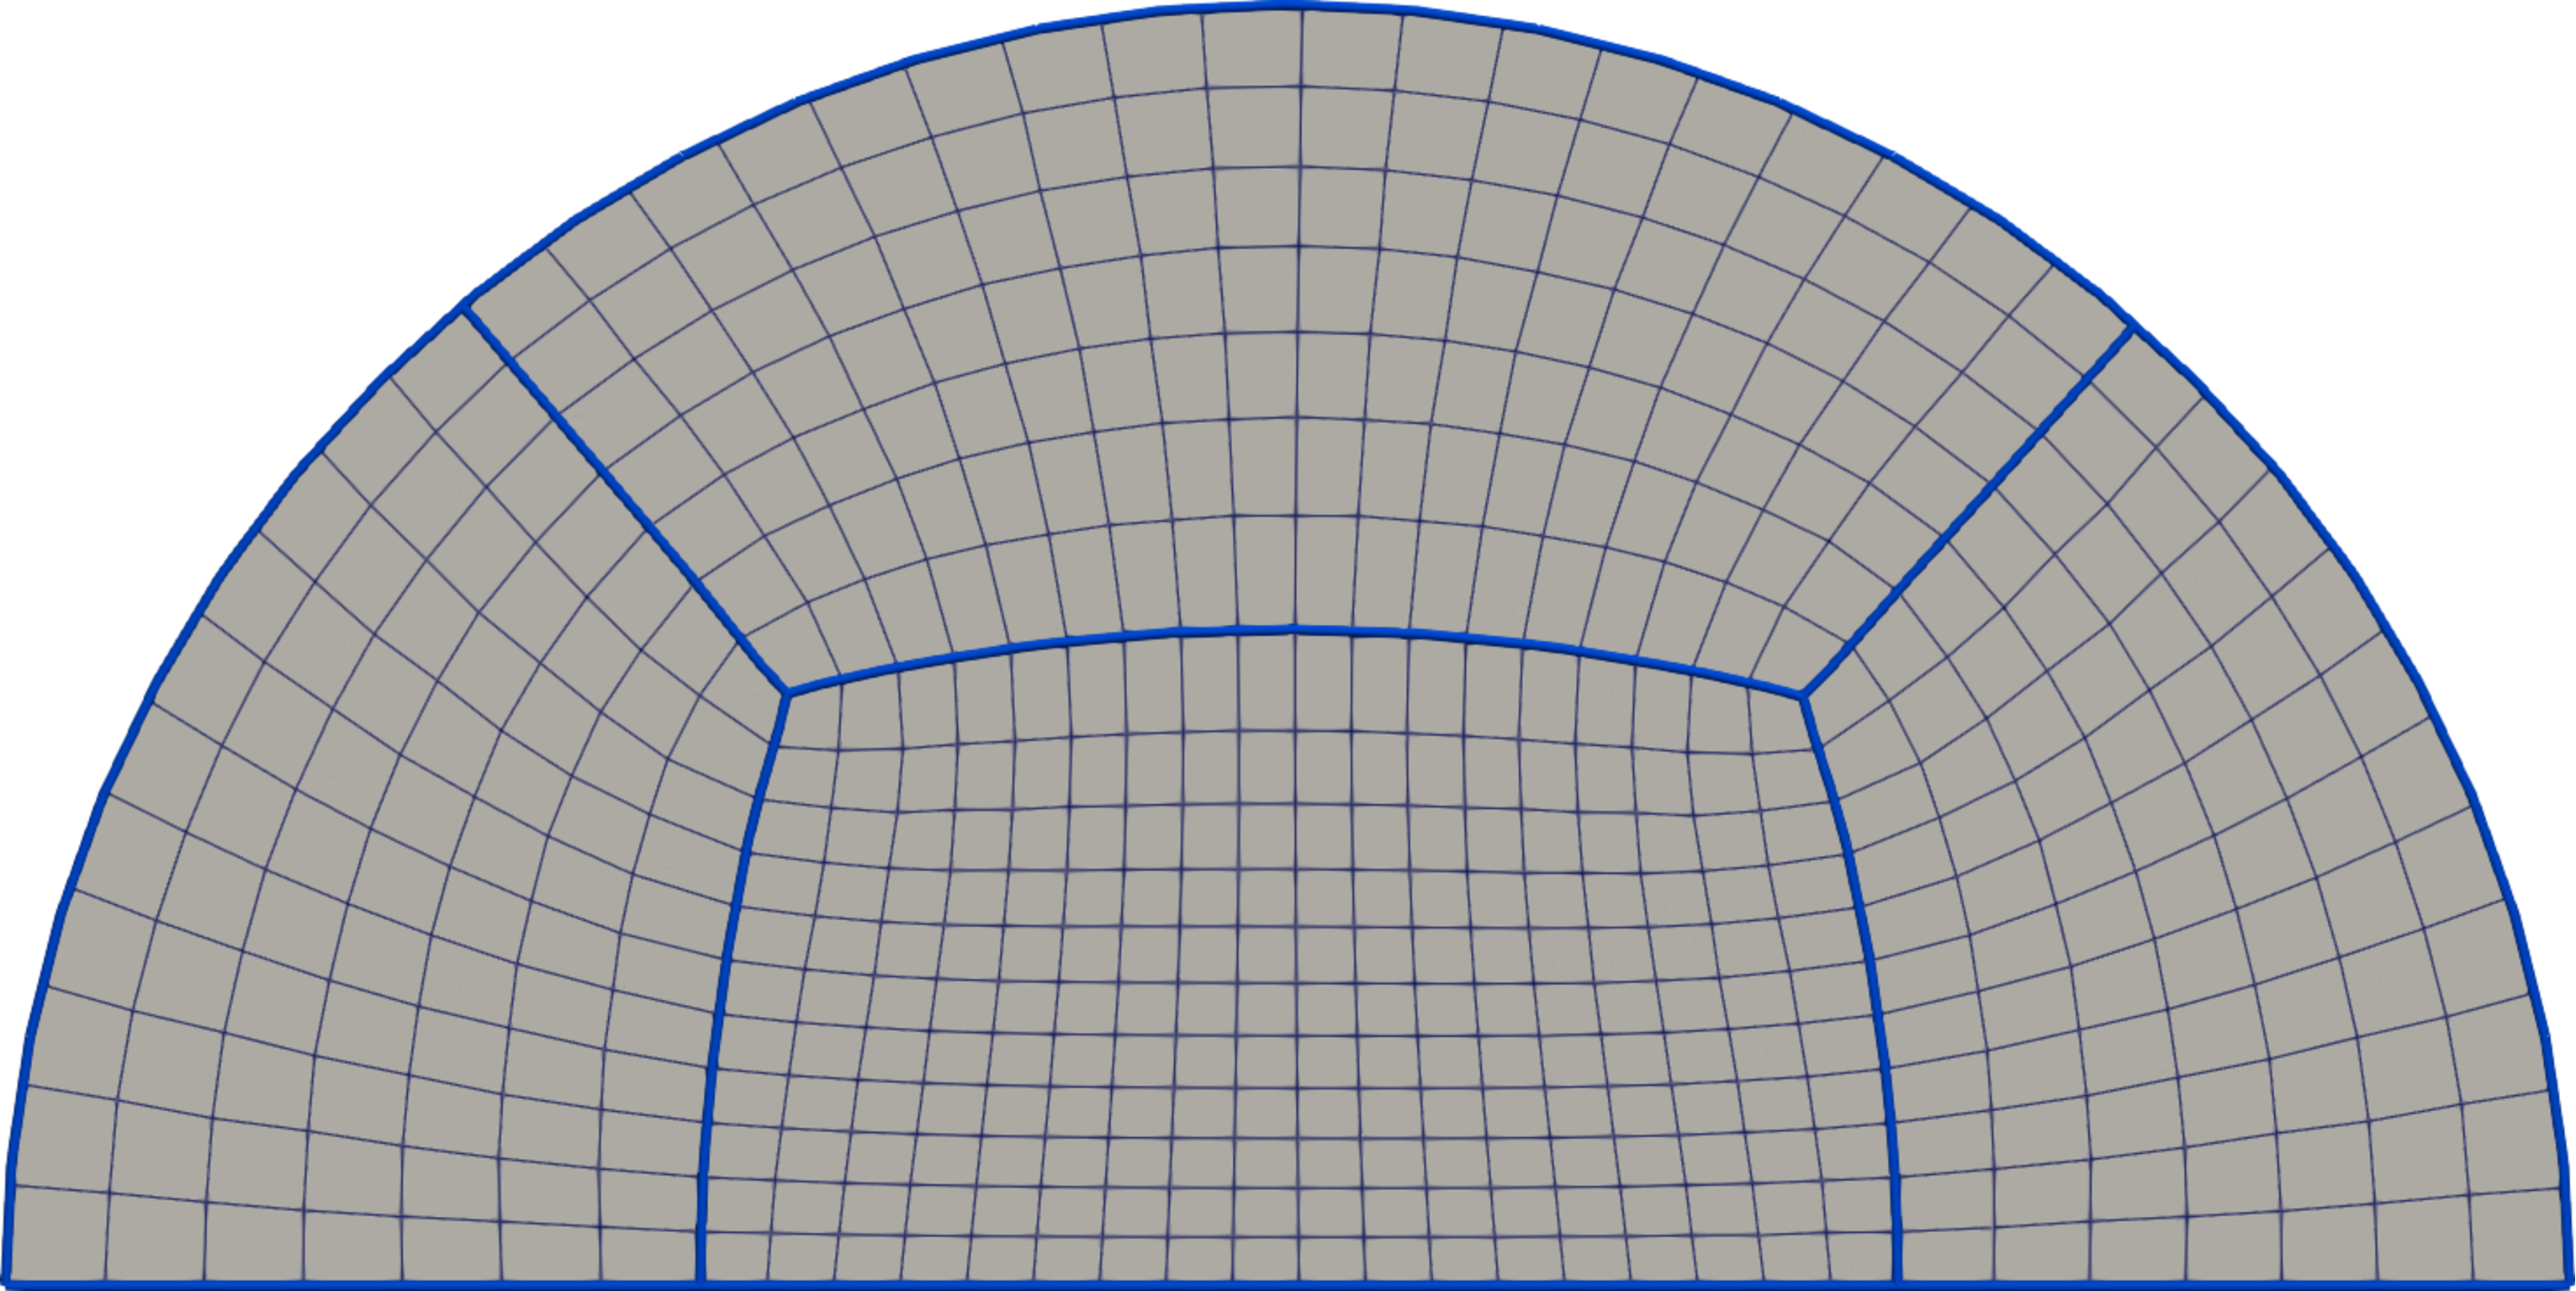
\includegraphics[width=\textwidth]{images/demi_disc_second_phi_second.pdf}
    \caption{fusion.}
    \label{fig:merge_sepa_third}
\end{subfigure}        
\caption{Illustration de l'opération d'alignement à partir du champ d'angle donné par l'équation \eqref{eqn:principe_def_phi}.}
\label{fig:merge_sepa}
\end{figure}


\subsection{Assemblage des partitions}

Une fois les séparatrices construites, le maillage triangulaire $\Omega_h$ sous-jacent à la méthode est divisé en plusieurs régions. Pour identifier ces régions, nous commençons par modifier $\Omega_h$ en un nouveau maillage. On récupère chaque région sous la forme d'un sous-maillage de $\Omega_h$ en faisant:
Localement dans chaque triangle,\\
on ajoute les points constituant les separatrices a $\Omega_h$ modifiant ainsi la topologie du maillage triangulaire initial,\\
Pour se faire, on exécute localement l'algorithme d'insertition de point localement dans chaque triangle.\\
donné par\\

\section{Opération d'alignement}

cos laplacien rtheta...
\[\]
Nous abordons maintenant la discrétisation de l'opération d'alignement présenté dans le chapitre \ref{chap:theoritical}. Étant donné une représentation $\bar{N}_h$ du champ de croix $\bar{N}$ sur le bord $\partial\Omega_h$ de $\Omega_h$, nous cherchons à modifier $\bar{u}_h$ en construisant un nouveau champ de croix $\bar{v}_h$ qui soit aligné avec $\partial\Omega_h$. Autrement dit, on veut que pour tout $p\in\partial\Omega_h$, $\bar{v}_h(p)\in\{\bar{N}_h(p), 0\}$. Pour se faire, on commence par définir l'ensemble des points singuliers de bord du champ de croix $\bar{v}$ que l'on note $\mathcal{B}$. On associe un paramètre $I_p$ pour tout $p\in\mathcal{B}$ représentant l'indice que nous souhaitons qu'il possède dans le champ de croix $\bar{v}$ et vérifiant:
\begin{equation}
I_p=
\left\{
\begin{array}{ll}
\displaystyle\frac{k}{4}\mbox{ avec }k\in\mathbb{Z}\mbox{ et }k\leq 1&\mbox{ si }p\in\mathcal{B},\\[0.5cm]
0&\mbox{ sinon }.
\end{array}
\right.
\end{equation}
Le champ de croix $\bar{u}_h$ choisit comme champ initial doit alors vérifié $0<\#\mathcal{S}_{\bar{u}_h}<\infty$ et pour tout point $p\in\mathcal{S}_{\bar{u}_h}$, $id_{\bar{u}_h}(p)=k/4$, avec $k\in\mathbb{Z}$ et $k\leq 1$. On suppose de plus que:
\begin{equation} 
    \label{eqn:etude_hyp_u_simple}
    \theta_{\bar{u}_h}-\theta_{\bar{u}_h}=\chi(\Omega)-\sum_{p\in\mathcal{B}}I(p).
\end{equation}
Le champ de croix $\bar{v}_h$ est alors donné par:
\begin{equation}
\bar{v}_h(p)=
\left\{
\begin{array}{ll}
\mathbf{R}(\phi_h(p))\bar{u}_h(p) & \mbox{ si } p\in\Omega_h\backslash(\mathcal{B}\cup\mathcal{S}_{\bar{u}_h}),\\[0.5cm]
\bar{N}_h(p) & \mbox{ si } p\in(\mathcal{S}_{\bar{u}_h}\cap\partial\Omega_h)\backslash\mathcal{B},\\[0.5cm]
0 & \mbox{ si } p\in\mathcal{B}.
\end{array}
\right.
\label{eqn:etude_def_v_second}
\end{equation}
où $\phi_h$ est une approximation de la fonction $\phi$ définie par l'équation de Laplace suivant:\begin{equation}
\left\{
\begin{array}{lcll}
\Delta\phi &=& 0 &\mbox{ dans }\Omega_h,\\[0.5cm]
\phi_h(\gamma(t))&=&\theta^\gamma_{\bar{N}_h}(t)+\mathcal{I}(t)-\theta_{\bar{u}_h}(\gamma(t)) & \mbox{ sur } \gamma^{-1}(\partial\Omega_h\backslash(\mathcal{B}\cup\mathcal{S}_{\bar{u}_h})),
\end{array}
\right.
\end{equation}
où $\gamma$ est une paramétrisation sur $[0, 1]$ de $\partial\Omega_h$ et la fonction $\mathcal{I}$ est donnée par:
$$
\mathcal{I}(t)=\displaystyle\sum_{s\in\gamma^{-1}(\mathcal{B})}\left[\left(\pi-\widehat{\gamma(s)}-2\pi I_{\gamma(s)}\right)-\left(\displaystyle\lim\limits_{r\rightarrow s^+}\theta^{\gamma}_{\bar{N}_h}(r) - \lim\limits_{r\rightarrow s^-}\theta^{\gamma}_{\bar{N}_h}(r)\right)\right]\mathbb{1}_{[0, t]}(s),
$$
avec $\widehat{\gamma(s)}$ la mesure de l'ouverture angulaire de la frontière en $\gamma(s)$.

ne pas oublié thetah pour le non-simplement connexe


\section{Etude de la méthode}

\subsection{Analyse de convergence}


\subsection{Lien entre $\bar{u}$ et $\bar{u}_h$}

\begin{lemma}
    $\mathcal{S}_{\bar{u}}=\mathcal{S}_{\bar{u}_h}$
\end{lemma}

Lorsque h tend vers 0, uh tend vers u\\

champ de croix u isolé donc uh isolé\\

vers quoi tend Qh ?\\

On se rend compte que les normales ne match pas.\\

Je me suis aligné avec les normales d'une autre géométrie. Laquelle?\\

On a eu Qh. \\

Lorsque h tend vers 0\\

Le partitionnement Qh obtenu suite au partitionnement est 'il une decomposisition en région de quatres côtés de $\Omega_h$ ?\\

En quel sens le partitionnement Qh obtenu est 


\section{Génération de champs de croix}
edp\\
z-ai\\
somme flux triangle

\section*{Construction d'un maillage quadrilatéral}
De manière similaire à ce qui a été exposé dans le chapitre précédent, nous entamons d'abord la mise en place du processus de partitionnement de $\Omega_h$, puis nous revenons sur la discrétisation des différentes méthodes permettant d'aligner un champ de croix donné sur le bord du domaine sur lequel il est défini. Pour finir, nous abordons le maillage en quadrangles des régions à quatre côtés résultant du partitionnement de $\Omega_h$.


\subsection*{Traitement des bords}

\subsection*{Obtention du maillage quadrilatéral}
Description de l'interpolation transfini.

\section*{Interprétation du partitionnement}
En vrai vh pas aligné avec omegah donc pas de raison que ca marche

vh tend vers v
Sh tend vers S
Rh tend R
chap 2 marche par v S et R donc partitionnement a 4 cotés
Donc Qh est un maillage de omega



Notons que le maillage $\Omega_h$ est construit de sorte que $\mathbf{B}$ soit inclut dans l'ensemble des sommets de $\partial\Omega_h$.\\

Jusqu'à présent, nous n'avons pas supposé que nous travaillions avec une discrétisation particulière. Dans ce chapitre, nous discrétisons la méthode sur des maillages triangulaires.

Dans le chapitre précédent, les composantes de premier plan mise en jeu sont: le domaine bornée $\Omega$, l'ensemble $\mathbf{B}$ des points de $\partial\Omega$ caractérisant la géométrie de $\Omega$ et le champ de croix initial $\bar{u}$ vérifiant l'hypothèse $\mathbf{H}_1$. Avec ces données, nous construisons un champ de croix $\bar{v}$ aligné avec le bord de $\Omega$ issue des différentes opérations abordés dans le chapitre précédent. $\bar{v}$ est ensuite utilisé pour partitionner le domaine $\Omega$ en régions de quatre côtés.

Commençons par exécuter le processus d'alignement sur le champ de croix $\bar{u}_h$ puisque le champ de croix $u$ dont il est l'approximation n'a aucune raison d'être aligné par rapport à $\Omega$. Pour se faire, nous cherchons un champ d'angle noté $\phi_h$ et vérifiant l'équation suivante:

\begin{equation}
\left\{
\begin{array}{lcl}
\Delta\phi_h &=& 0 \mbox{ dans }\Omega_h,\\[0.25cm]
\phi_h &=& \theta_{\Bar{N}_h}-\theta_{\bar{u}_h} \mbox{ sur } \partial\Omega_h.
\end{array}
\right.
\label{eq:phi_computation_omega_h}
\end{equation}

où $\bar{N}_h$ correspond au champ de croix de la normale extérieur de $\partial\Omega_h$. Remarquons que $\bar{N}_h$ est défini sur les arêtes de $\partial\Omega_h$ mais n'est pas défini sur les sommets de $\partial\Omega_h$. Autrement dit, le champ de croix $\bar{N}_h$ n'est pas compatible avec l'ensemble $\mathbf{B}$ puisque les points singuliers de $\bar{N}_h$ ne coïncident pas avec les points de l'ensemble $\mathbf{B}$. 

%Cela implique que suite au processus d'alignement, le champ de croix résultant $v_h=R(\phi_h)u_h$ aura comme point singulier de bord tous les sommets de $\partial\Omega_h$ autrement dit, les points singuliers de $\bar{v}_h$ ne coincideront pas avec les points de l'ensemble $\mathbf{B}$. Ainsi, un découpage  Le champ de croix $\bar{v}_h$ ainsi construit ne peut donc être une approximation du champ de croix $v$ dont les points singuliers correspondent à l'ensemble $\mathbf{B}$ (voir chapitre \ref{chap:theoritical}).

Pour palier à ce problème, nous modifions la définition du champ de croix normal. Supposons que l'on puisse définir un champ de croix $\widetilde{N}_h$ sur $\partial\Omega_h$ tel que les points singuliers de $\widetilde{N}_h$ correspondent exactement aux points de l'ensemble $\mathbf{B}$. L'équation \eqref{eq:phi_computation_omega_h} devient alors:

\begin{equation}
\left\{
\begin{array}{lcl}
\Delta\phi_h &=& 0 \mbox{ dans }\Omega_h,\\[0.25cm]
\phi_h &=& \theta_{\widetilde{N}_h}-\theta_{\bar{u}_h} \mbox{ sur } \partial\Omega_h.
\end{array}
\right.
\label{eq:phi_computation_omega_tilde}
\end{equation}

La résolution de l'équation \eqref{eq:phi_computation_omega_tilde} permet de construire le champ de croix $\bar{v}_h$ sur $\Omega_h$ définit par:
$$\bar{v}_h:p\in\Omega_h\longrightarrow \bar{v}_h(p)=\mathbf{R}(\phi_h(p))\bar{u}_h(p).$$

\newpage

On ne peut interpoler directement le champ de croix, on passe par un champ de vecteur intermédiare appelé champ de représentation \ref{},\\
\[\]
Cependant, il est clair que $\bar{v}_h$ n'est pas aligné avec $\partial\Omega_h$ puisque $\bar{v}_h=\widetilde{N}_h$ sur $\partial\Omega_h$. Autrement dit, le champ de croix $\bar{v}_h$ est aligné avec un domaine que nous notons $\widetilde{\Omega}_h$ et dont la normale extérieure est associé au champ de croix $\widetilde{N}_h$. $\bar{v}_h$ n'étant pas défini sur $\widetilde{\Omega}_h$ nous définissons une opération appelé \emph{lift} et noté $\mathbf{L}$ permettant de transporté une fonction définit sur un domaine vers un autre domaine. Nous désignons alors par $\widetilde{v}_h=\mathbf{L}_{\Omega_h}^{\widetilde{\Omega}_h}\bar{v}_h$ le lift de $\bar{v}_h$ de $\Omega_h$ vers $\widetilde{\Omega}_h$. Le champ de croix $\widetilde{v}_h$ ainsi défini est aligné avec $\partial\widetilde{\Omega}_h$ (bord de $\widetilde{\Omega}_h$) ce qui nous permet d'appliquer l'algorithme de partitionnement définit dans le chapitre \ref{chap:theoritical} à $\widetilde{v}_h$ sur $\widetilde{\Omega}_h$.

\subsection*{Définition de $\widetilde{N}_h$ et $\widetilde{\Omega}_h$}

\subsection*{Définition du Lift}

\subsection*{Discussion sur $Q_h$}

utiliser dans l'équation \eqref{eq:phi_computation_omega_h} en définissant le champ de croix $\widetilde{N}$ de la manière suivante:

$$
\forall p\in\partial\Omega_h,~~\widetilde{N}(p)=
\left\{
\begin{array}{lcl}
,\\[0.25cm]
.
\end{array}
\right.
$$

L'équation \eqref{eq:phi_computation_omega_h} devient alors:


Suite à la résolution de l'équation \eqref{eq:phi_computation_omega_tilde} sur $\Omega_h$, on peut construire le champ de croix $\bar{v}_h=\mathbf{R}(\phi_h)\bar{u}_h$ sur $\Omega_h$. On remarque alors que le champ de croix $\bar{v}_h$ ainsi construit n'est pas aligné avec $\Omega_h$.

\[\]
Définition de $\widetilde{\Omega}$

\begin{figure}[!h]
\centering
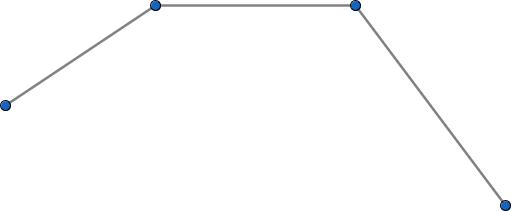
\includegraphics[scale=0.65]{images/Omega_h_tilde.png}
\caption{}
\label{fig:omega_h_tilde}
\end{figure}

\[\]
Définition du lift $\mathbf{L}$

\[\]
Définition de $\widetilde{v}=\mathbf{L}_{\Omega_h}^{\widetilde{\Omega}}v_h$

\[\]
Comparaison de $v$ et $\widetilde{v}$

\begin{eqnarray*}
\|v-\mathbf{L}_{\widetilde{\Omega}}^\Omega\widetilde{v}\|&\leq&\|\mathbf{R}(\phi)u-\mathbf{R}(\phi)\mathbf{L}_{\Omega_h}^\Omega u_h\|+\|\mathbf{R}(\phi)\mathbf{L}_{\Omega_h}^\Omega u_h - \mathbf{L}_{\widetilde{\Omega}}^\Omega\widetilde{v}\|\\
&\leq&\|\mathbf{R}(\phi)u-\mathbf{R}(\phi)\mathbf{L}_{\Omega_h}^\Omega u_h\|+\|\mathbf{R}(\phi)\mathbf{L}_{\Omega_h}^\Omega u_h - \mathbf{R}(\mathbf{L}_{\Omega_h}^\Omega\phi_h)\mathbf{L}_{\Omega_h}^\Omega u_h\|+\\
&&\| \mathbf{R}(\mathbf{L}_{\Omega_h}^\Omega\phi_h)\mathbf{L}_{\Omega_h}^\Omega u_h - \mathbf{L}_{\widetilde{\Omega}}^\Omega\mathbf{L}_{\Omega_h}^{\widetilde{\Omega}}v_h\|\\
&\leq&\|\mathbf{R}(\phi)u-\mathbf{R}(\phi)\mathbf{L}_{\Omega_h}^\Omega u_h\|+\|\mathbf{R}(\phi)\mathbf{L}_{\Omega_h}^\Omega u_h - \mathbf{R}(\mathbf{L}_{\Omega_h}^\Omega\phi_h)\mathbf{L}_{\Omega_h}^\Omega u_h\|+\\
&&\| \mathbf{R}(\mathbf{L}_{\Omega_h}^\Omega\phi_h)\mathbf{L}_{\Omega_h}^\Omega u_h - \mathbf{L}_{\widetilde{\Omega}}^\Omega\mathbf{L}_{\Omega_h}^{\widetilde{\Omega}}\mathbf{R}(\phi_h)u_h\|
\end{eqnarray*}



%\begin{figure}[!h]
%    \centering
%    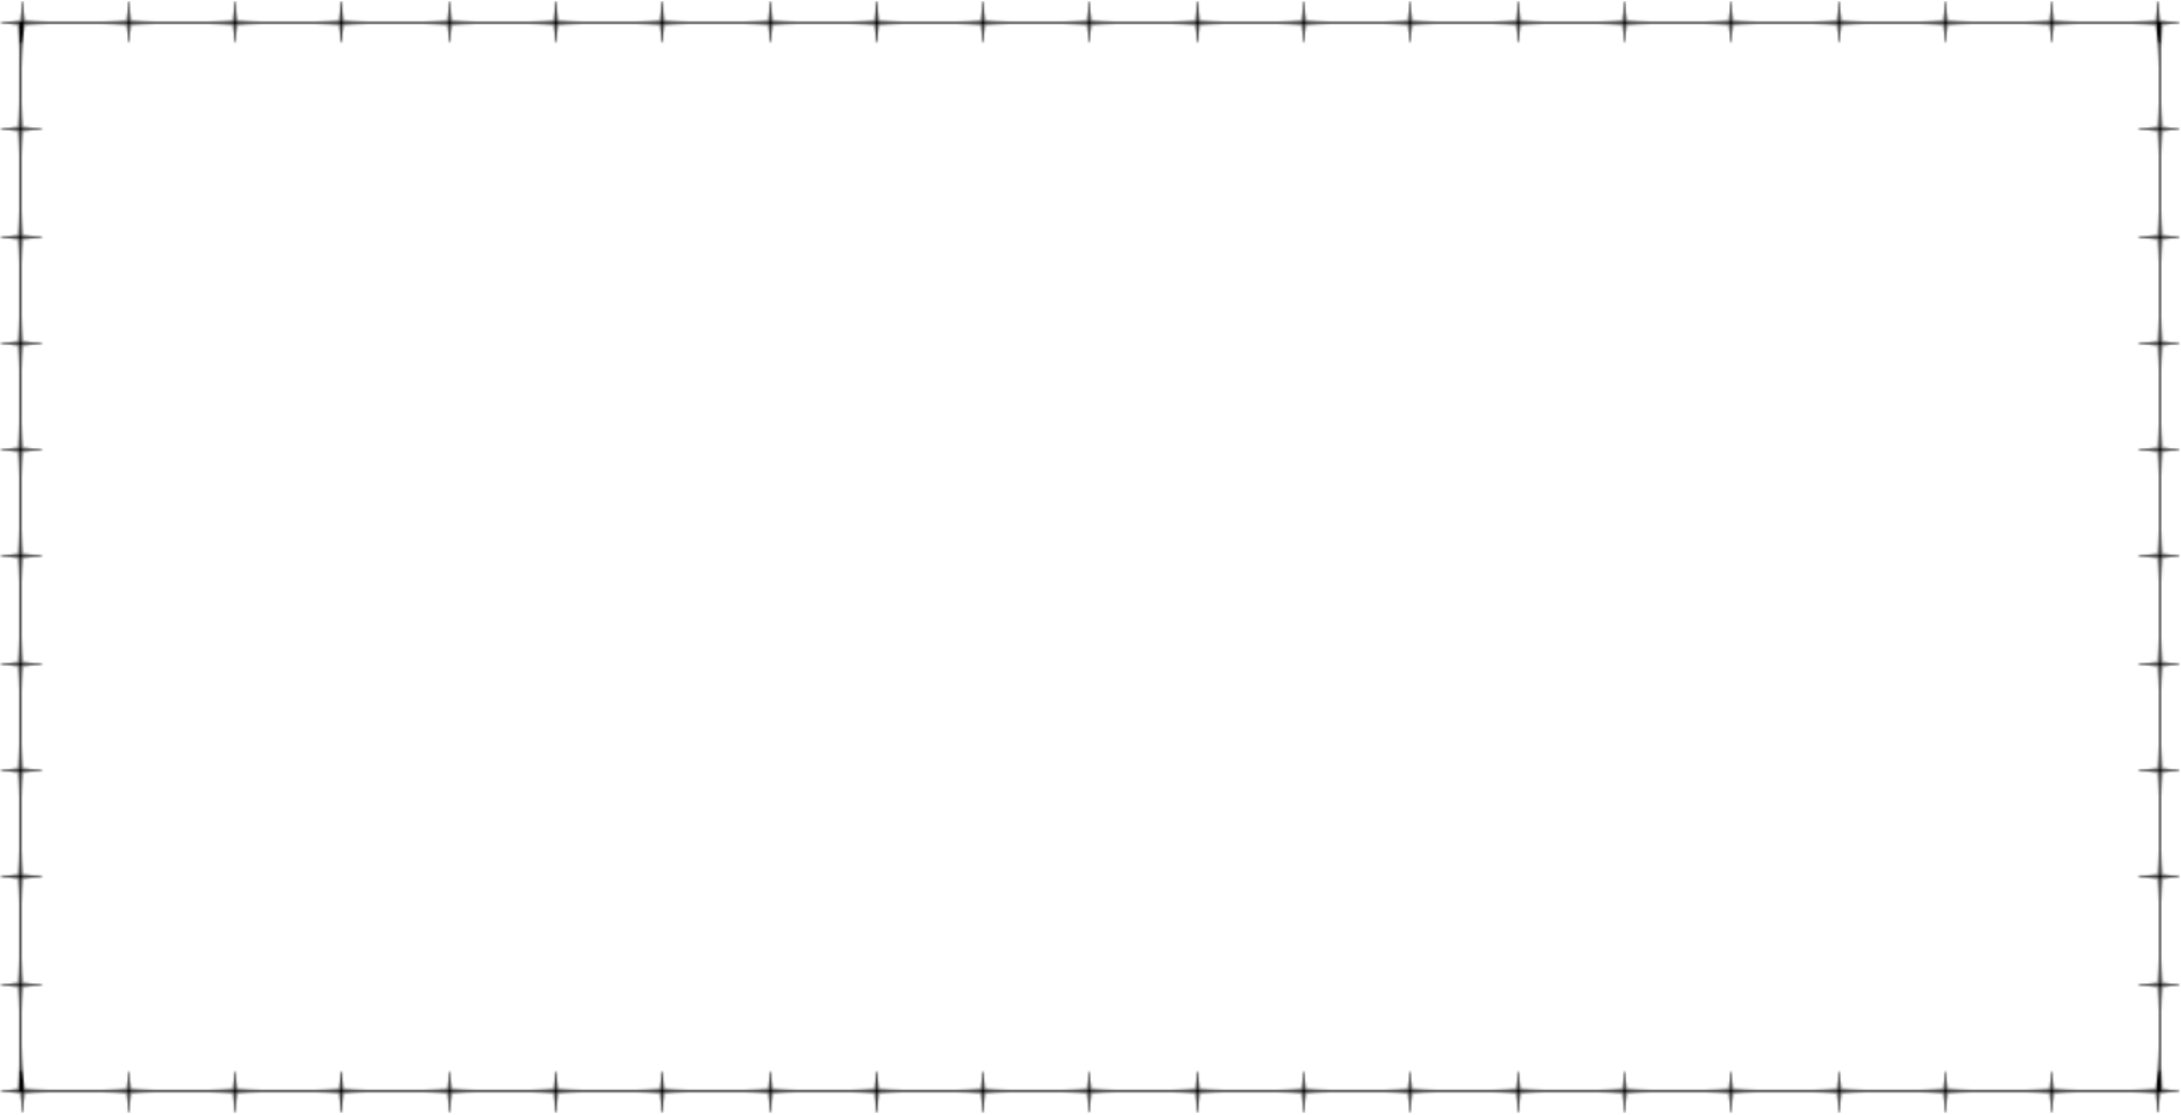
\includegraphics[scale=0.3]{images/im_default.pdf}
%    \caption{Maillage triangulaire d'un domaine quelconque}
%    \label{fig:mesh_tri_dom_quelc}
%\end{figure}
%Nous utilisons des tuples d'indices de sommets pour spécifier les simplices - par exemple, ijk est un triangle avec les sommets i, j, k ∈ V. Les indices apparaissant des deux côtés d'une équation sont fixés dans les sommes, par exemple ai j = Pi jk ∈ F bi jk signifie une somme uniquement sur les triangles ijk ∈ F contenant l'arête ij.

\section*{Algorithmes}
\color{blue}
remarque sur le tracé des "sreamlines" dans un triangle singulier en comparaison avec ce que fait viertel sachant que le champ n'est pas linéaire dans un tel triangle
\color{black}


\section*{Exemples}

\begin{figure}[!h]
\centering
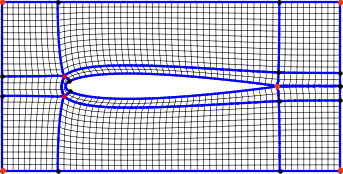
\includegraphics[scale=0.65]{images/nacas_normal.png}\hspace{0.5cm}
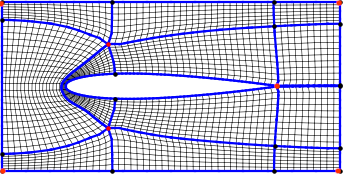
\includegraphics[scale=0.65]{images/naca_obus.png}
\caption{Mesh of Naca0012 with two different configurations of singular points. The initial cross-fields were obtained using formula (\ref{eq:z-ai}) .}
\label{connexe2}
\end{figure}

Structure de donnée\\
représentation des multimatériau\\


structure de donnée mesh
\[\]
generation champ de croix\\
discretisation par vertex\\
alignement champ de croix
\[\]
index\\
seul type 1 0 -1
\begin{figure}
    \centering
    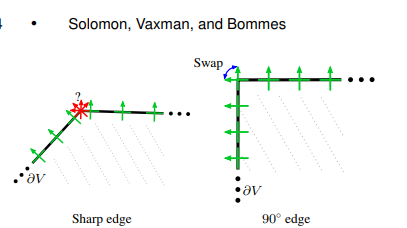
\includegraphics{images/inspi_1.png}
    \caption{Caption}
    \label{fig:enter-label}
\end{figure}

N'importe quel champ $\longrightarrow$  mesh quad\\*
preserver les points singuliers\\
Montrer simplement phi=N-U et sa trace\\
deplacer ensuite les singularité vers où ion veut

\[\]

Complementary Operations
Irregular Vertex Cancellation: We can move a v3 vertex to col-
lide with a v5 vertex, or vice versa, by applying multiple pair-wise
movement operations. When one v3 and one v5 vertex collide they
cancel each other and both become regular. At least one other ir-
regular vertex needs to be involved in this cancellation. In this fash-
ion we develop a 3 − 5 pair cancellation operation. It is possible
that the last step of a 3 − 5 pair cancellation is equivalent to one
3 − 3 − 5 − 5 removal operation and two pairs of irregular vertices
are canceled at once. Examples can be found in Figures 16 and 17.
Irregular Vertex Merging: A 3 − 3 pair can be merged to a v2
vertex and a 5 − 5 pair can be merged to a v6 vertex when their
graph distance is even. Theorems 7.2 and 7.3 provide the theoretical
analysis that is related to such a merge.
Irregular Vertex Alignment: Under the assumptions of Theo-
rems 7.2 and 7.3, arbitrary 3 − 3 and 5 − 5 pairs can be aligned
by applying multiple movement operations until d1 = 0 or d2 = 0.
Smoothing: We use iterative Laplacian mesh smoothing to im-
prove the geometry if the connectivity edits degrade the shape of
the mesh above a user-defined tolerance. The user can select uni-
form weights or cord-length weights, and elect to preserve sharp
features by constraining the positions of vertices on sharp edges.
The smoothing scheme can improve the aspect ratios of modified
faces. After each iteration all vertices are projected back onto the
original mesh. We have also experimented with a scheme in which
newly generated vertices are pulled towards vertices in the origi-
nal mesh if the distance between the new and original vertices is
above a threshold. The projection and pulling scheme can narrow
the difference to the original mesh. 
9 Connectivity Editing for Quadrilateral Meshes
Chi-Han Peng∗
Arizona State University
Eugene Zhang†
Oregon State University
Yoshihiro Kobayashi‡
Arizona State University
Peter Wonka§
Arizona State University /
KAUST